%SIGMETRICS
\documentclass{sig-alternate}

%USENIX
%\documentclass[letterpaper,twocolumn,10pt]{article}
%\usepackage{usenix,epsfig,endnotes}
%\usepackage{titlesec}
\usepackage{amsmath}
\usepackage[noend]{algpseudocode}
\usepackage{paralist,algorithm}
\usepackage{booktabs}
%\usepackage{subcaption}
\usepackage{multirow}
\usepackage{float}
\usepackage{graphicx}
\usepackage{pgfplots}
\usepackage{amssymb}
\usepackage{epstopdf}
\usepackage{tikz}
\usepackage{tkz-tab}
\usepackage{xspace}
%\usepackage{epsfig}
%\epstopdfsetup{outdir=./}
%\usepackage[showframe=true]{geometry}
\usepackage{enumitem}
\usepackage{adjustbox}
\usepackage[most]{tcolorbox}

\pgfplotsset{compat=1.10}


\addtolength{\columnsep}{-1.5mm}
\addtolength{\belowcaptionskip}{-1pt}
\setlength{\parskip}{3pt}
\setlength{\textfloatsep}{5pt}
%\topmargin=1pt
\topskip=1pt


\begin{document}

%USENIX
%\date{}

\title{\Large \bf Parikshan\xspace: Live Debugging of Production Systems in Isolation}

\iffalse
\author{
{Nipun Arora$^\dagger$, Franjo Ivan\v{c}i\'{c}}\\$^*$, Gail Kaiser$^\ddagger$}\\
$^\dagger$NEC Laboratories America \hspace{1.4cm}   $^\*$Google NYC \hspace{1.4cm}  $^\ddagger$Columbia University\\
nipun@nec-labs.com \hspace{4pt} ivancic@google.com \hspace{4pt} kaiser@cs.columbia.edu \\
}
\fi

%\iffalse
\author{
{Nipun Arora}\\
       NEC Labs\\
%       Princeton, NJ, USA\\
       nipun@nec-labs.com
\and
{Franjo Ivan\v{c}i\'{c}}\\
       Google NYC\\
%       New York, NY, USA\\
       ivancic@google.com
\and
{Gail Kaiser}\\
       Columbia University\\
%       New York, NY, USA\\
       kaiser@cs.columbia.edu
}
%\fi
\maketitle


\newcommand{\iprobe}{\texttt{iProbe}\xspace}
\newcommand{\parikshan}{\texttt{Parikshan}\xspace}
\newcommand{\livedebugging}{\textit{live debugging}\xspace}
\newcommand{\debugcontainer}{\textit{debug container}\xspace}
%\newcommand{\comment}[1]{}
\newtheorem{example}{Example}
\def\infinity{\rotatebox{90}{8}}

\begin{abstract}
  
%Existing Testing and Verification technologies, are impractical for testing large scale softwares. 
%One of the biggest problems faced by developers debugging large scale systems is replicating the deployed environment to figure out errors.
%Additionally, most modern companies are combining their development and operation management activities (DevOps), which has led to an increased emphasis on fast bug resolution.
%In recent years there has been a lot of work in record-and-replay systems which captures traces from live production systems, and replays them.
%However, most such record-replay systems have a high recording overhead and are still not practical to be used in production environments without paying a penalty in terms of user-experience. 
In this work we present a framework which allows users to debug a target production system (execution tracing, profile, breakpoint etc.) in a sandbox environment cloned from the live running system at any point in its execution.
% of a service oriented application. 
The paper leverages user-space containers (OpenVZ/LXC) to launch a container cloned and migrated from running instances of an application, thereby launching two containers: production (which provides the real output), and debug-container (for debugging). 
This \emph{debug-container} provides a sandbox environment for safe application of instrumentation tools without any perturbation to the actual production environment. 
%Test cases are initiated using user-defined probe points which launch test-cases using the execution context of the probe point. 
%Our sandboxes provide name-space, and resource management for the processes executing the test/debug cases.
A customized-network proxy agent replicates inputs from clients to both the production and debug-container, as well as safely discards all outputs from the debug-container.
%These sandboxed test-containers can be run either on the same physical host as the production container, or scaled out on dedicated physical test servers.
%, and manage the file system such that existing and newly created file descriptors are safely managed.
%Further we explain fidelity guarantees of our proposed system
We believe our tool provides a novel mechanism for practical live-debugging of large scale multi-tier and cloud applications, without requiring any application down-time, and minimal performance impact.
%In our evaluation provide a number of use-cases to show the utility of our tool.  
\end{abstract}


% A category with the (minimum) three required fields
%\category{H.4}{Information Systems Applications}{Miscellaneous}
%A category including the fourth, optional field follows...
\vspace{-2pt}
\category{D.2.5}{Testing \& Debugging}[debugging, tracing, monitoring]

%\terms{Theory}
\vspace{-2mm}
\keywords{software debugging, live cloning, network duplication}

\section{Introduction}
\label{sec:intro}

\begin{figure*}[ht!]
	\begin{center}
		%    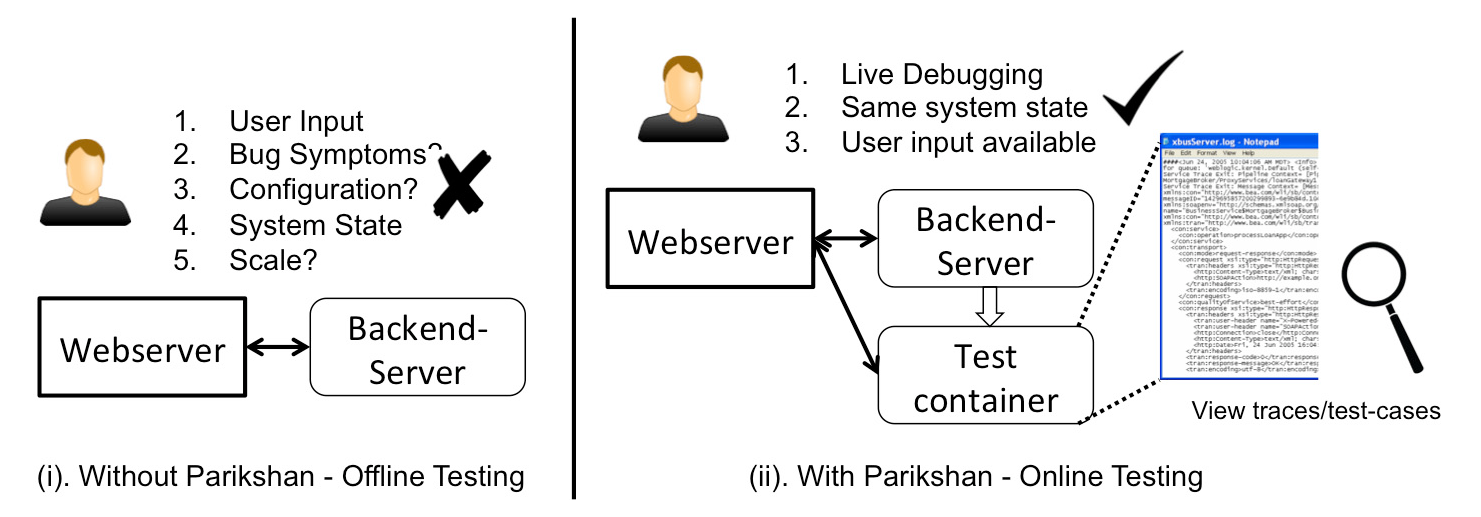
\includegraphics[width=0.7\textwidth]{figs/motivation.eps}
		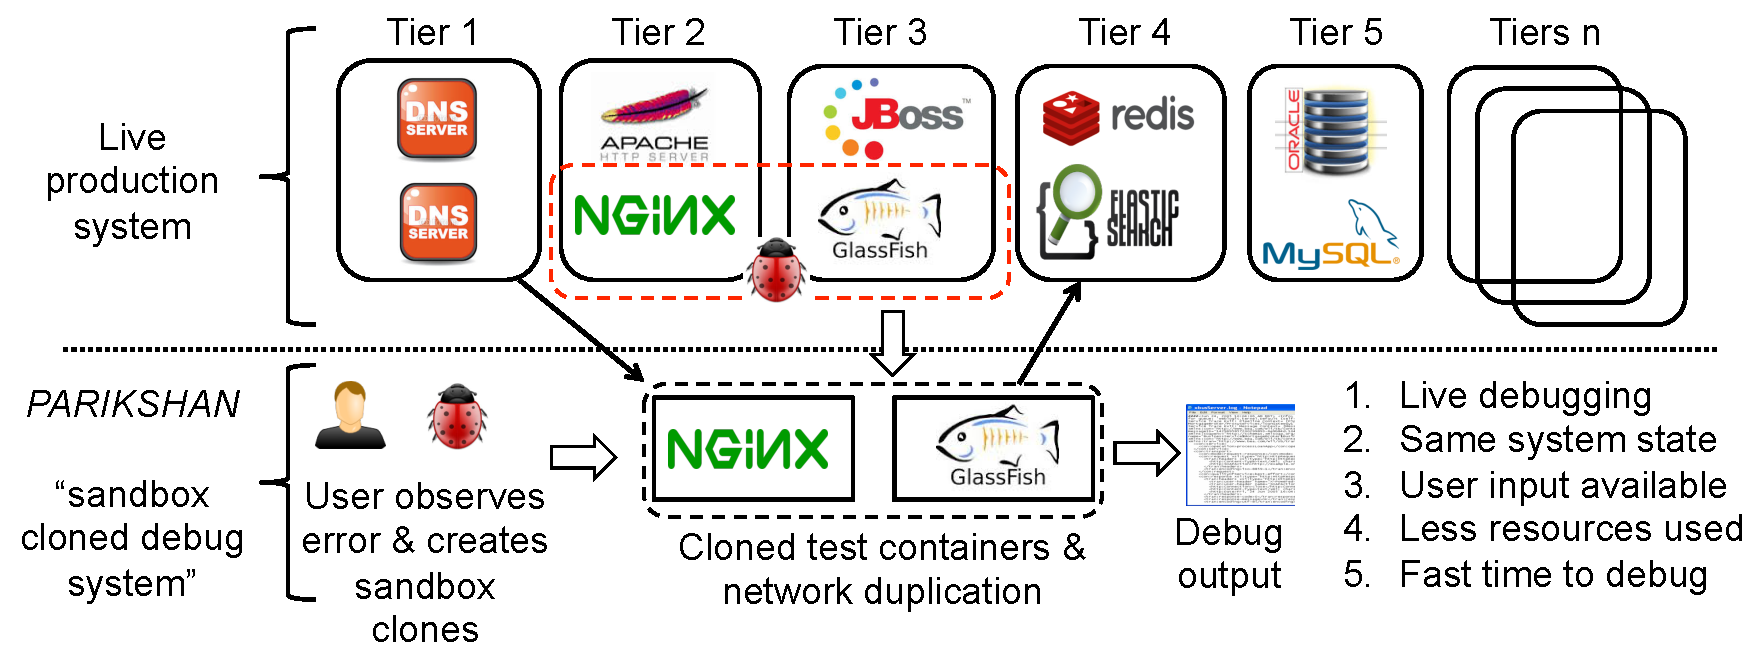
\includegraphics[width=0.9\textwidth]{figs/workflow3.pdf}
		\caption{Workflow of \parikshan in a live multi-tier production system with several interacting services. When the administrator of the system observes errors in two of it's tiers, he can create a sandboxed clone of these tiers and observe/debug them in a sandbox environment without impacting the production system.}
		\label{fig:motivation}
	\end{center}
\end{figure*}

Rapid resolution of incidence~(error/alert) management~\cite{sasase2013} in online service oriented systems is extremely important.
However, the complexities of virtualized environments coupled with large distributed systems have made bug localization harder. 
%The large scale of such systems means that any downtime has significant financial penalties for all parties involved.
On the other hand, there is a trend in the software engineering industry towards closer coupling between software developers and operators~(DevOps~\cite{devops}) in order to have shorter release and debug cycles 
(Facebook mobile has 2 releases a day, and Flickr has 10 deployment cycles per day~\cite{10DevOps}). 
%This re-emphasizes the need to have a very short time to diagnose and fix a bug.
Hence, debugging is hard not only because of difficulty to capture the root-cause, there is also an increased emphasis on the need to localize and fix bugs in a short period of time.

%Furthermore, whether to repair flaws or add features, software patches are released all the time.
%For instance, Facebook mobile has 2 releases a day, and Flickr has 10 deployment cycles per day~\cite{10DevOps}).
%Hence, it is increasingly important to localize and fix bugs in a very short period of time.
%As application software grows and gets more complicated, debugging large scale applications has become increasingly important. 
%This problem is further compounded by the recent trend in software engineering industry by large companies towards DevOps \cite{devops}. 
%The recent trend towards DevOps~\cite{devops} by the software engineering industry further compounds this problem. 
%by requiring a fast and rapid resolution towards any software bug.
%DevOps stresses on close coupling between software developers and operators, in order to have shorter release cycles (Facebook mobile has 2 releases a day, and Flickr has 10 deployment cycles per day~\cite{10DevOps}). 
%This re-emphasizes the need to have a very short time to diagnose and fix a bug.
%Hence, debugging is hard not only because of difficulty to capture the root-cause, it is also increasingly important to localize and fix bugs in a very short period of time.

Existing state-of-art techniques for monitoring production systems~\cite{dtrace, iProbe, winetw} rely on light-weight dynamic instrumentation to capture execution traces. 
Operators then feed these traces to analytic tools~\cite{magpie,clue} or do offline debugging, to find the root-cause of the error.
However, dynamic instrumentation has a trade-off between granularity of tracing and the performance overhead. 
Operators keep instrumentation granularity low, to avoid higher overheads in the production environment.
This often leads to multiple iterations between the debugger and the operator, to increase instrumentation in specific modules, in order to diagnose the root-cause of the bug. 
%To avoid higher overheads instrumentation granularity is generally kept low, thereby making bug diagnosis harder.
%Debugging is a lengthy process: debuggers try to piece together what could be the possible problem using log information.
%Often more information is required to understand the context better which leads to several iterations before the problem is debugged, thereby increasing the time-to-debug.

Another body of work has looked into record-and-replay~\cite{odr,revirt,laadan2010transparent,geels2007friday} systems which capture execution traces, in order to faithfully replay them in an offline environment.
These systems try to capture system level information, user-input, as well as all possible sources of non-determinism, to allow for in-depth \textit{post-facto} analysis of the error.
%Another tool, aftersight~\cite{aftersight} looks into recording, and replaying the execution in parallel, to allow for decoupled analysis. 
However, owing to the amount of instrumentation required, record-and-replay tools introduce an even heavier overhead. 
This may make them unacceptable for several user-facing systems where performance is essential.


%However, it is extremely difficult to meet the quick debugging demands of a devops environment, as it is not feasible to recreate realistic workloads in an offline development environment for large scale multi-tier or cloud based applications.
%\noindent
%Existing techniques for monitoring production systems~\cite{dtrace, iProbe, winetw} rely on light-weight dynamic instrumentation in either the kernel or the application. 
% kernel, application or error logs.  
%as a mechanism to localize and identify the bugs as well.
%There are several problems with these techniques:
%\begin{itemize}[leftmargin=*,topsep=0pt,itemsep=-1ex,partopsep=1ex,parsep=1ex]
%\textbf{Unrealistic} because 
%\item %These techniques rely on instrumentation to gather execution traces.
%Dynamic instrumentation has a trade-off between granularity of tracing and the performance overhead. 
%Operators usually avoid high instrumentation in live production system.
%Hence, the logs captured may not be enough to find root-cause of the error.
%\item Applications use a variety of third party plugins, are deployed on multiple kernels, which makes generating configurations and state of production systems difficult. 
 % traditional whitebox testing in the development environment is unable to capture these bugs.
%\item Debugging is a lengthy process: Developers try to piece together what could be the possible problem using log information.
%Often more information is required to understand the context better which leads to several iterations before the problem is debugged.
%\end{itemize}

%\noindent
%Recent work in record-and-replay~\cite{} tools allows operators to capture the context of the application and reproduce bugs in an offline environment.
%However, these tools incur a relatively high overhead, and can thereby not be used in production systems. 

%One of the proposed mechanisms of addressing this problem is to ``perpetually test''~\cite{perpetual} the application in the field after it has been deployed. 
%This is important since testing in a production system enables us to capture previously ``unreachable'' system states, which can arise due to various factors such as unpredictable user environment, outdated software, an ever increasing list of hardware devices (e.g. mobile phones, embedded devices etc.), or simply because of imperfect network connectivity (wifi, cellular).
%which are possible only for a long running production environment. 
%Since we are testing in a real environment, we get real user-input for test-cases, and are able to test a real environment.
%However, perpetual testing has never gotten much traction because of an obvious flaw : executing such test-cases will adversely effect the user-experience, both in performance and potentially in application logic.

%\noindent
%Previous approaches such as Chaos Monkey~\cite{chaosmonkey} from Netflix and AB Testing~\cite{abtesting} already use ``testing in the wild'' to check for errors and robustness of the software or to check for new features that have been added.  
%However, despite a clear need, debugging in the production environment has never gotten much traction in real-world applications as it may consume too much performance bandwidth and more importantly, it can impact the sanity\footnote{The state of the production server may change leading to a crash or wrong output} of real operational state of the software.
%Another trend embraced by mainstream companies such as Flickr, Twitter, Facebook and Google is DevOps\cite{devops}. 
%And wile testing, analyzing and monitoring are an important aspect of the devops cycle, usually only a very small performance bandwidth in the production server can be dedicated to QA operations as compared to real user activity(so as to not effect user-perceived delay). 

%Embedding test-case logic within the context of the application will result in state-change, or performance slow-down that would otherwise not be there in an optimized implmentation of the application.
%This is something which is usually unacceptable in user-facing applications.
%The authors have previously looked into amortizing the cost of running the test, by running it in parallel \cite{invite}.
%However such approaches cannot completely avoid the slowdown, and additonally do not completely sandbox the effects of the test case on the production server. 

%An alternate approach is to record live applications, and replay them offline.
%Over the years there have been several systems which have explored this direction with promising results.
%However most record and replay systems have high overheads, and require replication of the running configuration which may not be possible. 
%Additionally the administrator needs to wait for offline analysis, instead of doing real-time diagnosis.

%On the other hand, there has been an impressive increase in the scale of computing resources, and distributed scalability of infrastructure.
%Web based applications are often hosted in cloud environments, this allows for easily scaling up the hardware resources.
%This often allows for redundant computation, which can be used for testing purposes. 

%The main reason that debugging in the development environment is easier, is because developers can trace the execution flow of the program using tools such as gdb~\cite{gdb}, valgrind~\cite{valgrind} etc. and look at variable values for the given input. 
%This gives them an immediate insight as to whether the application is behaving correctly, and where the bug could be.
%Unfortunately, such techniques are not possible in the production environment as they would lead to unacceptable slow-down, alter the application functionality, or worse crash the application.

%The work aims to provide \textbf{``bug diagnosis as a service''} for real-time debugging and analysis of production applications, with no recording overhead on the production application.
%We observe that most modern day service oriented applications are hosted on IAAS cloud providers, and can hence be easily scaled  up. 
%Additionally, there have been rapid advances in user-space virtualization technologies such as Docker~\cite{docker}, and OpenVZ/LXC~\cite{openvz,lxc}, which allow users to easily launch and create light-weight application containers. 
%Check THIS LINE
%In particular, docker provides pre-installed containers(webservers, loadbalancers, appservers) which can be integrated together to create a service.
%Leveraging this abundance of resources, we present a debugging mechanism, which allows the user to dynamically insert probes in a \emph{cloned} production environment without impacting the actual application: thereby, enabling real-time diagnosis.

Our system, called \parikshan\footnote{\parikshan is the Sanskrit word for  testing}, allows \textbf{real-time debugging} without any performance impact on the production service. 
We provide a facility to sandbox the production and debug environments such that any modification in the debug environment does not impact user-facing operations.
%\parikshan can target specific sections of a running large scale distributed application, avoiding the need for a scaled out offline debugging cluster.
In particular, \parikshan allows system administrators to apply debugging techniques with deeper granularity instrumentation, without impacting performance or functionality.
For the remainder of this paper, we define \textbf{downstream servers} as servers from which requests are being sent to the production container, and \textbf{upstream servers} as servers to which the production container sends request. 
In Figure~\ref{fig:workflow}, the webserver is downstream, and the backend is upstream of our target container.

%We avoid recording overhead in the production container, while providing a facility for deeper bug diagnosis, and instrumentation.
%We have deployed \parikshan in  cloud infrastructure using user-space containers.

\parikshan leverages an abundance of resources available in the cloud environments to launch servers (debug containers) for the express purpose of debugging cloned from a running production system (production container). 
It is composed of three modules:
(a) a \textit{clone manager}, which manages cloning of production containers to debug containers.
(b) a \textit{network duplicator} module, which duplicates all incoming traffic from downstream servers to both production and debug containers.
(c) a \textit{network aggregator} module, which manages all communication from upstream servers to the debug-container.
The cloning operation is ``live'', hence there is no suspension of the services of the production server.
The debug container acts like a sandbox which restricts it from causing any perturbation to the state of the parent process, or impacting the sanity of the responses to the production client. 
This allows debuggers to use debugging tools without any fear of crashing or modifying the production application.

\iffalse
This is done by cloning an application container, and creating two containers: a production container, and a debug container. 
We duplicate incoming traffic from downstream servers to both production and debug containers.
Similarly, we have another module, which replays responses sent from the production container, to the debug container so that it is completely isolated from the network. 
The debugging on the debug-container is done on-the-fly using dynamic instrumentation tools like DTrace~\cite{dtrace}, or iProbe~\cite{iProbe}. 
%hence any set of test-cases can be turned on whenever required. 
%This is achieved by using dynamic instrumentation mechanisms to clone a VM by forking off from a running executed state and encapsulating the forked execution in a VM.
%The user can pre-define probe points for dynamically inserting test-cases (by default the entry and exit of each function is considered a probe point).
The cloned debug container acts like a sandbox which restricts it from causing any perturbation to the state of the parent process, or impacting the sanity of the responses to the production client. 
The cloning operation is ``live'', hence there is no suspension of the services of the production server.
\fi

\parikshan primarily focuses on non-crashing bugs~\cite{Zhang:2013:ADS:2486788.2486830, liu2005mining, kremenek2007factor}.
These bugs lead to either an inconsistent output or impact the performance of the application, without crashing the system.
Examples of such bugs are slow memory leaks, configuration errors, and performance bugs, which do not crash the application, but need to be fixed quickly to avoid degradation in service quality. 
Although many interesting methods have been developed to trace crashing bugs (memory violation, core dumps etc.), it is still difficult to analyze non-crashing bugs as they often happen in scaled out systems or because of difficult to reproduce edge-case scenarios.
%that are hard to replicate in unit tests or integration tests. 

We have deployed \parikshan in the context of cloud platform using user-space container virtualization technologies (OpenVZ/LXC~\cite{openvz,lxc}).
%A key insight of our design is that redundant resources often available in cloud infrastructures can be used for debugging purposes, while making the debugging process more efficient and reliable.
We assume that our target systems utilizes micro-service architectures (\texttt{Docker}~\cite{docker}), where each service (application, DNS, indexing, storage) is sandboxed in separate containers.
This allows us to launch debug-containers, which can target one application at a time.
Our techniques can also be applied to traditional VM's. 
However, containers are more light-weight, and utilize far less resources.
%While full VM virtualization has existed for several years, recent advances in user-space container technologies (OpenVZ/LXC~\cite{openvz,lxc}) has changed software engineering methodology. 
%Furthermore, container based technologies like \texttt{Docker}~\cite{docker} emphasize the use of micro-service architectures, where each service (application, DNS, indexing, storage) is sandboxed in separate containers. 


%In particular, there have been rapid advances in user-space virtualization technologies such as Docker~\cite{docker}, and , which allow users to easily launch and create light-weight application containers. 
%\textit{Parikshan}
%We provide a flexible framework which allows user access to a parallel test-container which behaves identically as the production container. 
%While we discuss several case-studies to debug/ test production applications that show how our framework can be used, we wish to stress that \textbf{the main advantage of \parikshan is a harness/ framework for testing/ debugging in a live environment rather than a new testing methodology}. 
\noindent
%\parikshan provides a facility for diagnosing bugs in containers cloned from a production system. 
The key contributions of our system are:
\begin{itemize}[leftmargin=*,topsep=0pt,itemsep=-1ex,partopsep=1ex,parsep=1ex]
\item \textbf{Sandbox debugging:} \parikshan provides a cloned sandbox environment to debug the production application.
This allows a safe mechanism to diagnose the error, without impacting the functionality of the application.
\item \textbf{No performance impact:} A network duplication and aggregation mechanism, which ensures non-blocking request duplication to the debug-container, thereby ensuring no performance impact on the application. 
\item \textbf{Capture large-scale context:} Allows to capture the context of large scale production systems, with long running applications. Under normal circumstances capturing such states is extremely difficult as they need a long running test input, and large test-clusters.
\item \textbf{Short time-to-debug:} These techniques contribute to a shortened debug time, by allowing users to directly gather trace data rather than wait for operators. 
%\item \textbf{Track debug container fidelity:} We track the fidelity of the debug-container (debug-container faithfully represents the production container). 
%and creates a flag whenever the containers are out-of-sync. 
%Parikshan debug-containers can tolerate some degree of divergence from the production state. 
%The debug-container may continue to run correctly even if the analysis run on it perturbs it's state slightly (it can tolerate some divergence from the production).
%The time till which the debug-container can faithfully represent the execution is called it's \emph{debugging -window} (see section \ref{sec:window}).
%\item We allow for \textbf{dynamic insertion of probes}, and safely capturing the execution trace of the application. 
%Dynamically inserting probes is important to avoid relaunching binaries in the test-container. 
%Restarting binaries would break active network connections, and destroy the in memory state of the test container(note: configuration/file-system state is still preserved).
%In our case studies we show how dynamic instrumentation mechanisms can be used with \parikshan

%\item One of the key advantages of our approach is that it is \textbf{language agnostic}. 
%Since the underlying mechanism takes advantage of containers as a platform to do the cloning, the language or interface does not matter as far as cloning is concerned. 
%Of-course testing mechanisms may differ depending upon different languages.
\end{itemize}


%\parikshan has been deployed on cloud IAAS platform using user-space container virtualization technologies (OpenVZ/LXC~\cite{openvz,lxc}).
%We tested \parikshan on several real world system, using realistic workloads.
\noindent
The rest of the paper is organized as follows.
In section~\ref{sec:motivation}, we describe a motivating scenario.
Section~\ref{sec:design} and \ref{sec:implementation} describe the design and implementation.
Next we discuss several real-world bugs(Section~\ref{sec:casestudy}), followed by the evaluation (Section~\ref{sec:evaluation}).
In Section~\ref{sec:application}, we discuss potential applications of \parikshan. 
Finally, we discuss some challenges(Section~\ref{sec:threats}), give some related work(Section~\ref{sec:related}) and conclude (Section~\ref{sec:conclusion}).

%\textbf{Virtual Machines vs Containers:} 
%Frequent synchronization is necessary because the test container can potentially go out of sync with the production because of non-determinism or because a test-case changes the state of the container, and effects future problems. 
%\textit{@Nipun edit -> consider why use user-space containers instead of VMs?}
%While VM virtualization has existed for several years, recent advances in user-space container technologies, along with support for migration, has created a space for light-weight testing in live environments.
%Technically our sandbox techniques could also be applied using more traditional Virtual Machines. 
%However, the overhead of using Virtual Machines is considerably higher, and it would technically require double the amount of resources for the target production servers.
%User-Space containers reduce this overhead considerably by using the resources in the same machine.
%We believe the availablity of resources in IAAS cloud infrastructures combined 
%\texttt{Zero-Probe Effect} probe points are added to the application which can be activated to insert test cases using ptrace~\cite{ptrace}.
%The use of dynamic instrumentation capability to add test cases in an application is an extension of our previous work of a dynamic instrumentation tool iProbe \cite{iProbe}
%Traditional testing approaches break states and are unable to  
%The authors previous work in in-vivo testing~\cite{invite} explored testing in the wild by initiating test cases in the production environment and sharing the load across several instances of deployed application.
%This approach adds test-cases in predetermined functions before starting the execution of the process, and periodically executes them in the run-time environment based on a probabilistic function. 
%\cite{dapper}


%\section{Motivation}

\subsection{Motivating Scenario}
\label{sec:motivation}

In Figure \ref{fig:motivation}, we have shown two workflows of the same system running with \parikshan, and without \parikshan.
To further explain, let us take  user Joe who is an administrator, and IT manager for a multi-tiered system. 
Much like several IT systems user Joe has a dashboard which informs him of the health status of all of his applications, and provides him with high level statistical views of all tiers of the system.
At time t0, Joe observes an unusually high memory usage by tier A for transaction type X or unusually high latencies in fetch operations for user Y (Alternatively, a trouble ticket could have been generated by the user).
Under usual circumstances, the system would have to go down(depending on the severity of the problem), the problem debugged using offline testing,  and the system would be patched once the problem has been diagnosed.
However often, it is difficult to find out the configuration of the system, and the user input which is causing this problem, also solving any emergent problems as soon as possible is extremely important.

Joe can now use \parikshan, to fork off a clone of \textit{tier A} as \textit{test-tier A}. 
Our proxy balancer sends a copy of the incoming request to \textit{test-tier A}, while users can continue using \textit{tier A}. 
The processes in \textit{test-tier A} follow the same execution paths, as they receive the same input as the production container(\textit{tier A}).
This allows Joe to initiate deeper test-cases, and observe the test-tier A, without fearing any problems in the user-facing operations.

% This paragraph needs serious revision - the points have been noted down but they need to be stated clearly in a better manner.
One of the key advantages of such an online approach is a reduced time to bug resolution.
Time to bug resolution is usually a very important criteria in any user-facing service oriented application, as the longer a bug remains the system, the more it is going to hit the user perception/revenue.
Bearing this in my mind we believe, that online testing will be an important aspect towards modern applications.
Additionally the usage of redundant computing for testing in A/B testing(see section \ref{sec:related}) approaches is a well accepted paradigm in real-world applications.
This leads us to believe that using redundant computing will be acceptable for regular testing approaches as well.

\iffalse
\subsection{Motivation Questions?}

To further motivate our testing paradigm we have come up with a set of motivating questions:

%\begin{compactitem}
%\setlength{\itemsep}{1Pt}
%\item[]\textbf{Q1:} Is it important to sandbox test-cases?
%\item[]\textbf{Q2:} Is recreating production environment difficult? 
%\item[]\textbf{Q3:} Is redundant computing available? 
%\item[]\textbf{Q4:} How would executing test-cases in a production server effect user-experience?
%\end{compactitem}

\subsubsection{\textbf{Q1:} Is it persistent testing important?}
\subsubsection{\textbf{Q2:} Is recreating production environment difficult?}
\subsubsection{\textbf{Q3:} Can redundant computing be utilized for testing?}
\subsubsection{\textbf{Q4:} How would executing test-cases in a production server effect user-experience?}
\fi
%\subsection{Impact}
\label{sec:impact}

The impact of sandbox testing can be seen in several different ways

\begin{itemize}
  \item \textbf{Sandbox Live Testing}
    One of the key motivations leading to \emph{Parikshan} is to provide a harness to allow the user to test real, live implementations. 


  \item \textbf{Fault Tolerance}
  \item \textbf{Verification}
  \item \textbf{Integration Testing}
\end{itemize}


%
\section{Introduction}
\label{sec:intro}

As application software grows and gets more complicated, debugging large scale applications has become increasingly important. 
%This problem is compounded by the recent trend in software engineering industry by large companies towards DevOps \cite{devops}. 
The recent trend towards DevOps~\cite{devops} by the software engineering industry further compounds this problem by requiring a fast and rapid resolution towards any software bug.
DevOps stresses on close coupling between software developers and operators, and to merge the operations of both. 
Most of these companies have very frequent releases and hence require a very short time to a bug fix, test, patch and release in order to realize continuous delivery (Facebook mobile has 2 releases a day, and Flickr has 10 deployment cycles per day~\cite{10DevOps}).
Hence, debugging is hard not only because of difficulty to capture the root-cause, it is also increasingly important to localize and fix bugs in a very short period of time.


\noindent
However, it is extremely difficult to meet the quick debugging demands of a devops environment, as it is not feasible to recreate realistic workloads in an offline development environment for large scale multi-tier or cloud based applications.
Existing techniques for monitoring production systems~\cite{dtrace, iProbe, winetw} rely on light-weight dynamic instrumentation in either the kernel or the application. 
% kernel, application or error logs.  
%as a mechanism to localize and identify the bugs as well.
There are several problems with these techniques:
\begin{itemize}[leftmargin=*,topsep=0pt,itemsep=-1ex,partopsep=1ex,parsep=1ex]
%\textbf{Unrealistic} because 
\item These techniques rely on instrumentation to gather execution traces.
Dynamic instrumentation has a trade-off between granularity of tracing and the performance overhead. 
Operators usually avoid high instrumentation in live production system.
Hence, the logs captured may not be enough to find root-cause of the error.
\item Applications use a variety of third party plugins, are deployed on multiple kernels, which makes generating configurations and state of production systems difficult. 
 % traditional whitebox testing in the development environment is unable to capture these bugs.
\item Debugging is a lengthy process: Developers try to piece together what could be the possible problem using log information.
Often more information is required to understand the context better which leads to several iterations before the problem is debugged.
\end{itemize}

%\noindent
%Recent work in record-and-replay~\cite{} tools allows operators to capture the context of the application and reproduce bugs in an offline environment.
%However, these tools incur a relatively high overhead, and can thereby not be used in production systems. 

One of the proposed mechanisms of addressing this problem is to ``perpetually test''~\cite{perpetual} the application in the field after it has been deployed. 
%This is important since testing in a production system enables us to capture previously ``unreachable'' system states, which can arise due to various factors such as unpredictable user environment, outdated software, an ever increasing list of hardware devices (e.g. mobile phones, embedded devices etc.), or simply because of imperfect network connectivity (wifi, cellular).
%which are possible only for a long running production environment. 
%Since we are testing in a real environment, we get real user-input for test-cases, and are able to test a real environment.
%However, perpetual testing has never gotten much traction because of an obvious flaw : executing such test-cases will adversely effect the user-experience, both in performance and potentially in application logic.
%\noindent
Previous approaches such as Chaos Monkey~\cite{chaosmonkey} from Netflix and AB Testing~\cite{abtesting} already use ``testing in the wild'' to check for errors and robustness of the software or to check for new features that have been added.  
However, despite a clear need, debugging in the production environment has never gotten much traction in real-world applications as it may consume too much performance bandwidth and more importantly, it can impact the sanity\footnote{State of server may change leading to crash or wrong output} of real operational state of the software.
%Another trend embraced by mainstream companies such as Flickr, Twitter, Facebook and Google is DevOps\cite{devops}. 
%And wile testing, analyzing and monitoring are an important aspect of the devops cycle, usually only a very small performance bandwidth in the production server can be dedicated to QA operations as compared to real user activity(so as to not effect user-perceived delay). 

%Embedding test-case logic within the context of the application will result in state-change, or performance slow-down that would otherwise not be there in an optimized implmentation of the application.
%This is something which is usually unacceptable in user-facing applications.
%The authors have previously looked into amortizing the cost of running the test, by running it in parallel \cite{invite}.
%However such approaches cannot completely avoid the slowdown, and additonally do not completely sandbox the effects of the test case on the production server. 

%An alternate approach is to record live applications, and replay them offline.
%Over the years there have been several systems which have explored this direction with promising results.
%However most record and replay systems have high overheads, and require replication of the running configuration which may not be possible. 
%Additionally the administrator needs to wait for offline analysis, instead of doing real-time diagnosis.

%On the other hand, there has been an impressive increase in the scale of computing resources, and distributed scalability of infrastructure.
%Web based applications are often hosted in cloud environments, this allows for easily scaling up the hardware resources.
%This often allows for redundant computation, which can be used for testing purposes. 

%The main reason that debugging in the development environment is easier, is because developers can trace the execution flow of the program using tools such as gdb~\cite{gdb}, valgrind~\cite{valgrind} etc. and look at variable values for the given input. 
%This gives them an immediate insight as to whether the application is behaving correctly, and where the bug could be.
%Unfortunately, such techniques are not possible in the production environment as they would lead to unacceptable slow-down, alter the application functionality, or worse crash the application.

\noindent
The motivation behind our work is to provide \textbf{``bug diagnosis as a service''} for real-time debugging of production applications in order to significantly reduce the time towards bug resolution.
%We observe that most 
Most modern day service oriented applications are hosted on IAAS cloud providers, and can hence be easily scaled  up. 
Additionally, there have been rapid advances in user-space virtualization technologies such as Docker~\cite{docker}, and OpenVZ/LXC~\cite{openvz,lxc}, which allow users to sandbox and ship application containers. 
%Check THIS LINE
%In particular, docker provides pre-installed containers(webservers, loadbalancers, appservers) which can be integrated together to create a service.
Leveraging this abundance of resources we present a debugging mechanism which allows the user to dynamically insert probes in a \emph{cloned} production environment without impacting the actual application: thereby, enabling real-time diagnosis.

\noindent
Our system called \parikshan\footnote{\parikshan is the Sanskrit word for testing}, allows capturing the context of application, and debugging to to done without impacting the sanctity and performance of the actual user-facing application. 
This is done by cloning a production server and creating two containers: a production container, and a debug container. 
We duplicate the incoming traffic to both the production container and the debug container using a custom proxy, which ignores the responses from the debug-container.
Similarly, we have another module which replays responses sent to the production container, to the debug container so that it is completely isolated as far as network communication is concerned. 
The debugging on the debug-container is done on-the-fly using dynamic instrumentation. %hence any set of test-cases can be turned on whenever required. 
%This is achieved by using dynamic instrumentation mechanisms to clone a VM by forking off from a running executed state and encapsulating the forked execution in a VM.
%The user can pre-define probe points for dynamically inserting test-cases (by default the entry and exit of each function is considered a probe point).
The cloned debug container acts like a sandbox which restricts it from causing any perturbation to the state of the parent process, or impacting the sanity of the responses to the production client. 
The cloning operation is ``live'', hence there is no suspension of the services of the production server.

%\textit{Parikshan}
%We provide a flexible framework which allows user access to a parallel test-container which behaves identically as the production container. 
%While we discuss several case-studies to debug/ test production applications that show how our framework can be used, we wish to stress that \textbf{the main advantage of \parikshan is a harness/ framework for testing/ debugging in a live environment rather than a new testing methodology}. 
\noindent
The key contributions of this paper are:
\begin{itemize}[leftmargin=*,topsep=0pt,itemsep=-1ex,partopsep=1ex,parsep=1ex]
\item A novel mechanism which significantly \textbf{reduces the time to debug} errors, by allowing debuggers to directly get information rather then wait for operators.
\item A tool which provides a sandbox environment to debug the production environment. 
This allows for a safe and secure mechanism to perturb and diagnose the application, \textbf{without effecting the functionality} of the  production container.
\item A testing harness, and proxy which ensures non-blocking request duplication to the debug-container, which ensures \textbf{no performance impact} on the production container. 
\item Allows to \textbf{capture the context} of large scale production systems, with long running applications. Under normal circumstances capturing such states is extremely difficult as they need a long running test input, and run on large test-clusters.
\item We track the \textbf{fidelity of the debug-container} (debug-container faithfully represents the production container). 
%and creates a flag whenever the containers are out-of-sync. 
The time till which the debug-container maintains fidelity is called it's \emph{debugging -window}( see section \ref{sec:window}).
%\item We allow for \textbf{dynamic insertion of probes}, and safely capturing the execution trace of the application. 
%Dynamically inserting probes is important to avoid relaunching binaries in the test-container. 
%Restarting binaries would break active network connections, and destroy the in memory state of the test container(note: configuration/file-system state is still preserved).
%In our case studies we show how dynamic instrumentation mechanisms can be used with \parikshan

%\item One of the key advantages of our approach is that it is \textbf{language agnostic}. 
%Since the underlying mechanism takes advantage of containers as a platform to do the cloning, the language or interface does not matter as far as cloning is concerned. 
%Of-course testing mechanisms may differ depending upon different languages.

\end{itemize}

\noindent
\textbf{Virtual Machines vs Containers:} 
While full VM virtualization has existed for several years, recent advances in user-space container technologies has changed software engineering methodology. 
In particular applications like \texttt{Docker} have emphasized the use of micro-service architectures, where each service (such as the application, dns, indexing, or storage) is sandboxed in separate containers. 
This allows developers to isolate each software and spin off containers at ease.
While \parikshan can be applied to traditional virtual machines, we believe that containers are more light-weight(less resouce usage), and lend themselves better to our design.
%Frequent synchronization is necessary because the test container can potentially go out of sync with the production because of non-determinism or because a test-case changes the state of the container, and effects future problems. 
%\textit{@Nipun edit -> consider why use user-space containers instead of VMs?}
%While VM virtualization has existed for several years, recent advances in user-space container technologies, along with support for migration, has created a space for light-weight testing in live environments.
%Technically our sandbox techniques could also be applied using more traditional Virtual Machines. 
%However, the overhead of using Virtual Machines is considerably higher, and it would technically require double the amount of resources for the target production servers.
%User-Space containers reduce this overhead considerably by using the resources in the same machine.
%We believe the availablity of resources in IAAS cloud infrastructures combined 
%\texttt{Zero-Probe Effect} probe points are added to the application which can be activated to insert test cases using ptrace~\cite{ptrace}.
%The use of dynamic instrumentation capability to add test cases in an application is an extension of our previous work of a dynamic instrumentation tool iProbe \cite{iProbe}
%Traditional testing approaches break states and are unable to  
%The authors previous work in in-vivo testing~\cite{invite} explored testing in the wild by initiating test cases in the production environment and sharing the load across several instances of deployed application.
%This approach adds test-cases in predetermined functions before starting the execution of the process, and periodically executes them in the run-time environment based on a probabilistic function. 
%\cite{dapper}


%\section{Motivation}

\subsection{Motivating Scenario}
\label{sec:motivation}

In Figure \ref{fig:motivation}, we have shown two workflows of the same system running with \parikshan, and without \parikshan.
To further explain, let us take  user Joe who is an administrator, and IT manager for a multi-tiered system. 
Much like several IT systems user Joe has a dashboard which informs him of the health status of all of his applications, and provides him with high level statistical views of all tiers of the system.
At time t0, Joe observes an unusually high memory usage by tier A for transaction type X or unusually high latencies in fetch operations for user Y (Alternatively, a trouble ticket could have been generated by the user).
Under usual circumstances, the system would have to go down(depending on the severity of the problem), the problem debugged using offline testing,  and the system would be patched once the problem has been diagnosed.
However often, it is difficult to find out the configuration of the system, and the user input which is causing this problem, also solving any emergent problems as soon as possible is extremely important.

Joe can now use \parikshan, to fork off a clone of \textit{tier A} as \textit{test-tier A}. 
Our proxy balancer sends a copy of the incoming request to \textit{test-tier A}, while users can continue using \textit{tier A}. 
The processes in \textit{test-tier A} follow the same execution paths, as they receive the same input as the production container(\textit{tier A}).
This allows Joe to initiate deeper test-cases, and observe the test-tier A, without fearing any problems in the user-facing operations.

% This paragraph needs serious revision - the points have been noted down but they need to be stated clearly in a better manner.
One of the key advantages of such an online approach is a reduced time to bug resolution.
Time to bug resolution is usually a very important criteria in any user-facing service oriented application, as the longer a bug remains the system, the more it is going to hit the user perception/revenue.
Bearing this in my mind we believe, that online testing will be an important aspect towards modern applications.
Additionally the usage of redundant computing for testing in A/B testing(see section \ref{sec:related}) approaches is a well accepted paradigm in real-world applications.
This leads us to believe that using redundant computing will be acceptable for regular testing approaches as well.

\iffalse
\subsection{Motivation Questions?}

To further motivate our testing paradigm we have come up with a set of motivating questions:

%\begin{compactitem}
%\setlength{\itemsep}{1Pt}
%\item[]\textbf{Q1:} Is it important to sandbox test-cases?
%\item[]\textbf{Q2:} Is recreating production environment difficult? 
%\item[]\textbf{Q3:} Is redundant computing available? 
%\item[]\textbf{Q4:} How would executing test-cases in a production server effect user-experience?
%\end{compactitem}

\subsubsection{\textbf{Q1:} Is it persistent testing important?}
\subsubsection{\textbf{Q2:} Is recreating production environment difficult?}
\subsubsection{\textbf{Q3:} Can redundant computing be utilized for testing?}
\subsubsection{\textbf{Q4:} How would executing test-cases in a production server effect user-experience?}
\fi
\subsection{Impact}
\label{sec:impact}

The impact of sandbox testing can be seen in several different ways

\begin{itemize}
  \item \textbf{Sandbox Live Testing}
    One of the key motivations leading to \emph{Parikshan} is to provide a harness to allow the user to test real, live implementations. 


  \item \textbf{Fault Tolerance}
  \item \textbf{Verification}
  \item \textbf{Integration Testing}
\end{itemize}


%

%\section{Motivation}

\subsection{Motivating Scenario}
\label{sec:motivation}

In Figure \ref{fig:motivation}, we have shown two workflows of the same system running with \parikshan, and without \parikshan.
To further explain, let us take  user Joe who is an administrator, and IT manager for a multi-tiered system. 
Much like several IT systems user Joe has a dashboard which informs him of the health status of all of his applications, and provides him with high level statistical views of all tiers of the system.
At time t0, Joe observes an unusually high memory usage by tier A for transaction type X or unusually high latencies in fetch operations for user Y (Alternatively, a trouble ticket could have been generated by the user).
Under usual circumstances, the system would have to go down(depending on the severity of the problem), the problem debugged using offline testing,  and the system would be patched once the problem has been diagnosed.
However often, it is difficult to find out the configuration of the system, and the user input which is causing this problem, also solving any emergent problems as soon as possible is extremely important.

Joe can now use \parikshan, to fork off a clone of \textit{tier A} as \textit{test-tier A}. 
Our proxy balancer sends a copy of the incoming request to \textit{test-tier A}, while users can continue using \textit{tier A}. 
The processes in \textit{test-tier A} follow the same execution paths, as they receive the same input as the production container(\textit{tier A}).
This allows Joe to initiate deeper test-cases, and observe the test-tier A, without fearing any problems in the user-facing operations.

% This paragraph needs serious revision - the points have been noted down but they need to be stated clearly in a better manner.
One of the key advantages of such an online approach is a reduced time to bug resolution.
Time to bug resolution is usually a very important criteria in any user-facing service oriented application, as the longer a bug remains the system, the more it is going to hit the user perception/revenue.
Bearing this in my mind we believe, that online testing will be an important aspect towards modern applications.
Additionally the usage of redundant computing for testing in A/B testing(see section \ref{sec:related}) approaches is a well accepted paradigm in real-world applications.
This leads us to believe that using redundant computing will be acceptable for regular testing approaches as well.

\iffalse
\subsection{Motivation Questions?}

To further motivate our testing paradigm we have come up with a set of motivating questions:

%\begin{compactitem}
%\setlength{\itemsep}{1Pt}
%\item[]\textbf{Q1:} Is it important to sandbox test-cases?
%\item[]\textbf{Q2:} Is recreating production environment difficult? 
%\item[]\textbf{Q3:} Is redundant computing available? 
%\item[]\textbf{Q4:} How would executing test-cases in a production server effect user-experience?
%\end{compactitem}

\subsubsection{\textbf{Q1:} Is it persistent testing important?}
\subsubsection{\textbf{Q2:} Is recreating production environment difficult?}
\subsubsection{\textbf{Q3:} Can redundant computing be utilized for testing?}
\subsubsection{\textbf{Q4:} How would executing test-cases in a production server effect user-experience?}
\fi
\section{Design}
\label{sec:design}

%In this section we begin with an explanation of live cloning to explain to the reader some the key challenges in designing a sandbox. We then give a system overview of \texttt{Parikshan}, explaining each of its components. 
%Next, we explain how it inserts test cases, into the test harness, and finally we explain how a user can use the \texttt{Parikshan} api to insert test cases in the test harness.

\begin{figure}[t]
  \begin{center}
    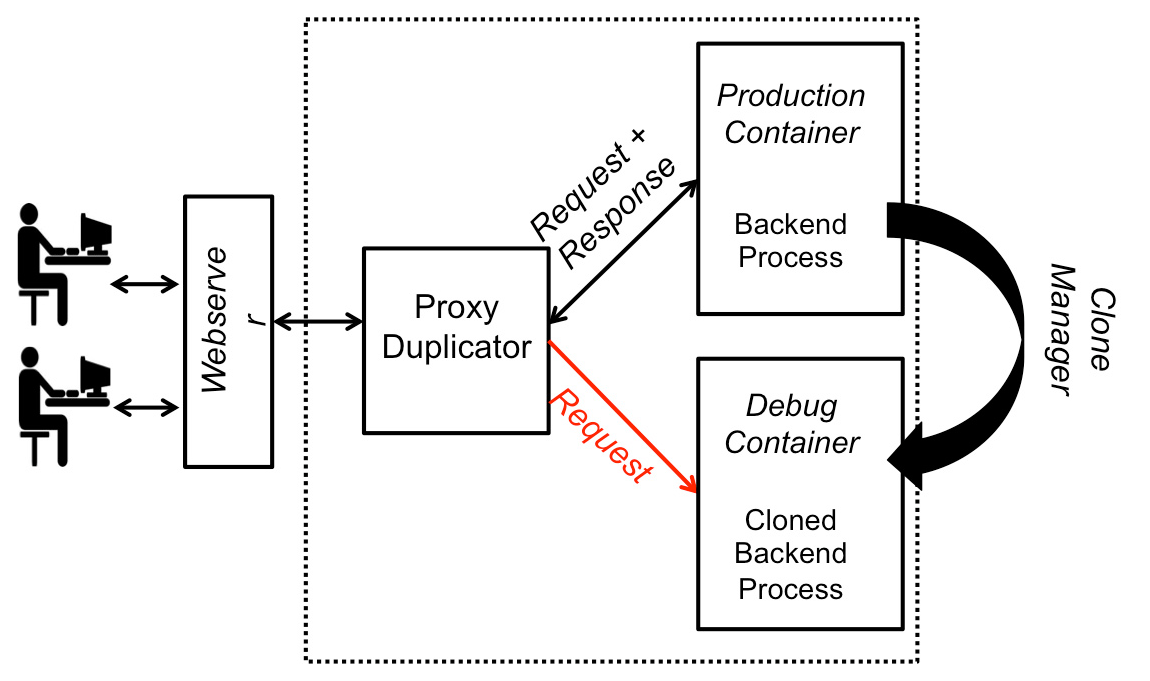
\includegraphics[width=0.45\textwidth]{figs/workflow2.eps}
    \caption{Backend wrapped around with Parakishan Run-time}
    \label{fig:workflow}
  \end{center}
\end{figure}

%\subsection{Workflow and Architecture}
%\label{sec:workflowArch}

%The basic workflow of \textit{Parikshan} is as described in Figure \ref{fig:workflow}. 
%\textit{Parikshan} can be applied at the boundary of every tier of a multi-tier system. In figure \ref{fig:workflow} we show parikshan being applied to a single tier boundary( communication from a webserver to a backend server) to showcase a simple example, this process can be easily scaled depending on the complexity of the system design. 
%The architecture is driven by a proxy request duplication agent( see section \ref{ and a live clone manager.

\subsection{System Overview}
\label{sec:systemOverview}

Each instance of \textit{Parikshan} can target only one tier at a time.
However, multiple instances can be orchestrated together especially when it's required for integration testing or cross tier results need to be correlated.
To begin with let us look at a simple example of client webserver with a database server as the backend (as shown in Figure \ref{fig:workflow}), where the test harness needs to be applied on the backend.
As explained earlier basic workflow of our system is to duplicate all network requests to the production backend server and a ``live cloned'' test container.
Traffic duplication is managed by our proxy network duplicator (see section \ref{sec:proxyDuplicator}), which uses several different strategies to clone user input to our test-container, with minimal impact on the production container.
Another core aspect of our design is how to implement ``live cloning''; this is the process by which a production container (in this case our backend service), can be cloned to create a test-container which has the same file system and process state. 
Cloning and syncing between the production container and the test-container is managed by our clone manager, which uses user-space containers OpenVZ and a variant of live migration to manage the cloning.
Next, we explain each of the modules in detail.
%The architecture can be divided into two parts: (1) A Proxy Network Duplicator, (2) container clone manager

%\begin{itemize} 

\subsection{Clone Manager} 
\label{sec:CloneManager}

\subsubsection{How does cloning work?}
\label{sec:cloning}

While the focus of our work is not to support VM Container migration, or to make changes to the hypervisor, we need to tweak the way typical hypervisors offer live migration for our purposes.
Before moving further we wish to clarify that instead of the standard live migration supported by hypervisors, \textit{Parikshan} requires a cloning functionality. 
In contrast with live migration, where a container is copied to a target destination, and then the original container is destroyed, the cloning process requires both containers to be actively running, and be still attached to the original network.
This cloning requires some tweaking, and modification in both how compute migration is handled, and especially how the network migration is handled. 

To understand cloning in our context, let us understand how live migration works. 
Live migration refers to the process of moving a running virtual machine, guest os or container from one host node(physical machine) to another, without disconnecting any client or process running within the machine. 
Live migration is supported by most well known Hypervisors( vmware, virtualbox, xen, qemu, kvm) with different amount of efficiency.
There are several variants of migration, some of which require a short suspend time, while others are able to seamlessly transfer without any noticeable down-time by the user.
In general the process involves the following steps: 
(1) Firstly, the copy (\textit{rsync}) is initiated by a pre-copy memory migration, where the underlying hypervisor copies all the memory pages from the source to the destination. 
(2) Once pre-copy phase is finished, the VM is temporarily suspended, and all memory pages including live memory pages are transferred to the target node. 
Once all memory pages have been transferred the target container is restarted. 
Obviously, two rsync runs are needed, so the first one moves most of the data, while the container is still up and running, and the second one moves the changes made during the time period between the first rsync run and the VM stop
\footnote{Network migration is managed by the IAAS which publishes the same MAC address for the copied VM. 
Since the identity of the target container remains the same, the IAAS is able to give it same IP Address, and network traffic is rerouted after the identity is published in the network}.
%To reduce the down-time memory pages are transferred probabiliticly based on priority, and incase a page is not found a network fault is generated which executes a fetch from the original VM.

Instead of Live Migration, in Live Cloning, we do not suspend operations of the source container, rather we allow the container to keep executing in both production and test locations.
The more tricky aspect is that there are two containers with the same identities in the network and application domain. 
This is important, as the operating system and the process may be configured with the IP Address, or other networking operation, which cannot be changed without leading to a crash of the system.
Hence the same network identifier should map to two seperate addresses.
Clearly the same ipAddress, mac addresses cannot be kept for both the production and test-container as that would lead to conflict in the network. 
There are two ways to resolve this : 
(1) Host each container behind their own network namespaces, on the same host machine, and configure packet forwarding to both containers such that the duplicator can communicate to them. 
Network namespaces(see internal mode, figure.\ref{fig:modesCloning}) is a definete possiblity, and have been used by several hosting providers, to launch VM's with same private ipAddress, in a shared network domain \cite{OpenStack}. 
(2) Another approach is to host both containers in different machines with port forwarding setup to forward incoming TCP requests to containers behind a NAT (see external mode, figure.\ref{fig:modesCloning}). 
This is slightly more scalable and has clear seperation of network and compute resources. 
However, an obvious downside to this approach is that it needs a new VM to be allocated.
This leads us to two different modes of implementation, which we discuss in the next section.
%As of now, we have implemented the second approach for our proof of concept mostly because of the ease of implementation.
%Further a packet level sniffer or mirror port would keep the same buffer and potentially timeout.
%To allow for some load-balancing and an application aware buffer, we went for a web application level proxy server to duplicate traffic to both containers. 
%
%Further in this section we explain how we deal with these challenges.

\subsubsection{Basic Design \& Modes}

The Clone Manager itself is just an interface which interacts with an \textit{agent} installed in each container host.
The clone manager dictates the frequency of cloning/syncing operations, as well as  coordinates setup operations/orchestration etc.
The agent itself is the driver for live cloning, and performs rsync operations, snapshot, transferring and starting the image.

\begin{figure}[t]
  \begin{center}
    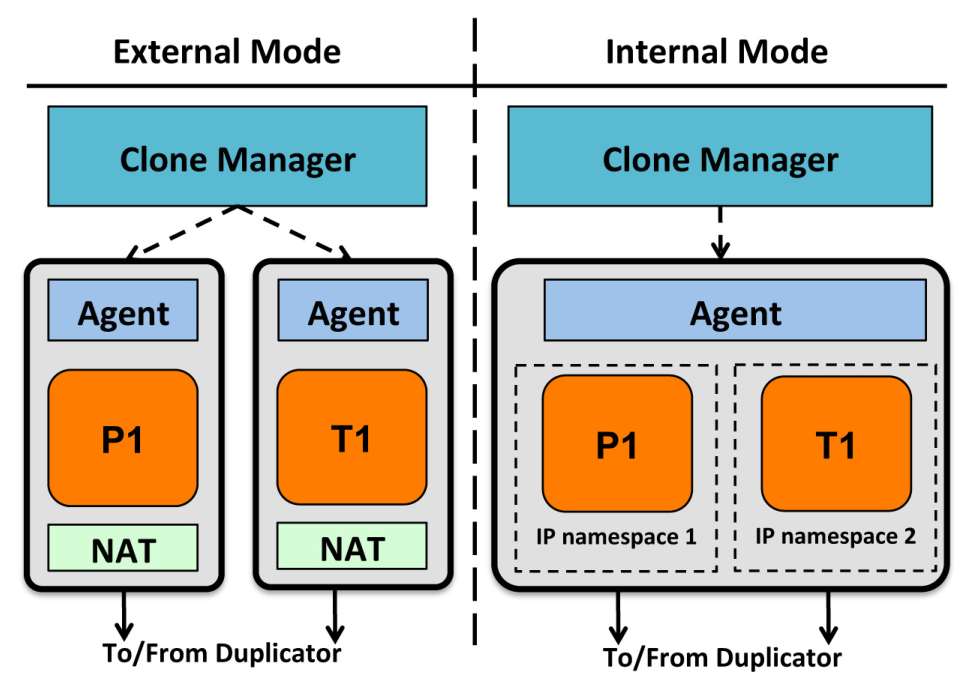
\includegraphics[width=0.5\textwidth]{figs/modesCloning.eps}
    \caption{External and Internal Mode for Live Cloning: P1 is the production container, and T1 is the test container, the Clone Manager interacts with an Agent which has drivers to implement live Cloning}
    \label{fig:modesCloning}
  \end{center}
\end{figure}


Test and production containers can be allocated in various schemes: we call these schemes \textit{modes}. 
Broadly speaking the clone manager works in 2 modes (see figure.\ref{fig:modesCloning}) : 
\begin{itemize}

\item \textit{Internal Mode}: In this mode we allocate the test-container and  production containers to the same host node. 
This would mean less suspend time, as the production container can be locally cloned ( instead of streaming over the network). 
Requires the same amount of resources as the original production container (number of host nodes remain the same), hence could potentially be cost-effective.
On the down-side, co-hosting the test and production containers, could have an adverse effect on the performance of the production container, hence effecting the user.
As we can see in figure.\ref{fig:modesCloning} the production container P1 and test container T1 are both hosted within the same physical host, and with the same ip addres, but their network is encapsulated within different network namespaces to sandbox them.
The duplicator is then able to communicate to both these containers with no networking conflict.

\item \textit{External Mode}: In this mode we provision an extra VM as the host of our test-container (this VM can host more than one test-containers), 
While this mechanism can have a higher overhead in terms of suspend time (~3 seconds, dependent on process state), and it will require provisioning an extra host-node, the advantage of this mechanism is that once cloned, the VM is totally seperate and will not effect the performance of the production-container.
We believe that such a mode will be more benificial in comparison to the internal mode, as testing is likely to be transient, and it is often more important to not effect user experience\footnote{ \textit{Scaled Mode}: This can be viewed as a variant of the External Mode, where we can scale out test-containers to several testing containers which can be used to do statistical testing and distribute the instrumentation load to capture the overhead easier. This reduces the frequency with which the container needs to be synced. This is currently out of the scope of this paper, however we aim to show this in a future publication.}.
As we can see in figure.\ref{fig:modesCloning} the production container P1 and test container T1, are hosted on two different host machines, and are encapsulated behind a NAT\cite{nat} (network address translator), hence they each have their ip's in an internal network thereby avoiding any conflict.

\end{itemize}

%\RestyleAlgo{boxruled}
%\LinesNumbered

%\\ \\
%\noindent \textbf{Implementation}\\
\subsubsection{Implementation}
%The Clone Manager is responsible for creating a live running ``clone'' of the production container and launch it as the test-container. 
%In our current setup cloning is done for each target production environment in the same physical host machine (we can clone to a different physical host as well, however for optimization purposes we have assumed that they will always be in the same local network).
In our current implementation, we are using OpenVZ\cite{openvz} as our container engine, and have modified the migration mechanism in vzctl \cite{vzctl} to make it work for live cloning instead. 
We tested this out on multiple VM's acting as host nodes for OpenVZ containers. 
To make the cloning easier and faster, we used OpenVZ's \textit{ploop} devices \cite{ploop} to host the containers. 
\textit{Ploop} devices are a variant of disk loopback devices where the entire file system of the container is stored as a single file. 
This makes features such as syncing, moving, snapshots, backups and easy seperation of inodes of each container file system.

The algorithm for live cloning is explained below: 

\begin{algorithm}[ht]
   \caption{Algorithm for Live Cloning using OpenVZ 
   \label{algCloning}}
 \begin{enumerate}
   \item Safety Checks(Checks that a destination server is available via ssh w/o entering a password, and version checking of OpenVZ running in it) 
   \item Runs rsync of container file system (\textit{ploop} device) to the destination server  
   \item Checkpoints and suspend the container 
   \item Runs a second rsync of the \textit{ploop} device to the destination  
   \item Start container locally 
   \item Set up port forwarding and packet duplication
   \item Starts the container on the destination 
  \end{enumerate}
\end{algorithm}

Let us imaging we are cloning production container C1 on Host H1 as test container C2 on Host H2. 
The initial setup requires certain safety checks and pre-setup to ensure easy cloning, these include: ssh-copy-id operation for accessing without password, checking pre-existing container ID's, check version of vzctl etc. 
These ensure that H1 and H2 are compatible, and ready for live-cloning.
Next, we run an intial rsync of container C1, from Host H1 to Host H2, this step does not require any suspension of C1, and copies the bulk of the container file system to the destination server (H2). 
The next step involves checkpointing, and dumping the process in memory state to a file, this is what allows the container to be restarted from the same checkpointed state. 
However for sanity of the container process, it is important to restart the container from the same file system state as it was when the checkpoint was taken.
To ensure this, we take a second rsync of the ploop device of C1, and sync it with H2, after this the original container can be restarted.
Next we copy the dump file from step 3, from H1 to H2, and resume a new container from that dump file.

Clearly the overhead of live migration depends on the I/O operations happening within the container between step 2 and step 4 (the first and the second rsync), as this will directly impact the amount of memory that needs to be copied during the suspend phase. 
A few iteration of cloning a container back and forth between two OpenVZ instances ( on KVM's within the same physical machine), resulted in an average suspend time of 1.8 seconds for the production container, and 3.3 seconds for launch of the test-container( see table \ref{table:clonePerf}).
%add citation for OpenVZ Live Migration performance iteration testbed http://openvz.livejournal.com/47780.html
This is nearly the same as that of native live migration\cite{openvzLiveMigrationPerf}, and has lesser suspend time for the production container as we do not include the \textit{``copy dump file''}, or the \textit{``undump and resume phase''} for production containers. 

%The same amount of resources as the production container are reserved for the test-container. 
%After doing the pre-copy, we do a pause for syncing the two containers, and start them together. 
%Subsequent clone operations are optimized as they only require rsync for the change that has happened to the base image and in memory operation.
%After the intial setup, the frequency of cloning depends on the slowdown experienced by the test-container, and requirement of the test-case (some test cases may not require a long running test-window).

\begin{table}[t]
  \centering
    \begin{tabular}{ | p{2.2cm} | l | l | l | l | l | l | l |}
    \hline
    \textbf{Iteration} & \textbf{1} & \textbf{2} & \textbf{3} & \textbf{4} & \textbf{5} & \textbf{Avg} \\ \hline
    \textbf{Suspend + Dump} & 0.60 & 0.60 & 0.57 & 0.74 & 0.59 & 0.65\\ \hline
    \textbf{Pcopy after suspend} & 0.60 & 0.60 & 0.57 & 0.74 & 0.59 & 0.65\\ \hline
    \textbf{Copy Dump File} & 0.60 & 0.60 & 0.57 & 0.74 & 0.59 & 0.65\\ \hline
    \textbf{Undump and Resume} & 0.60 & 0.60 & 0.57 & 0.74 & 0.59 & 0.65\\ \hline
%    \textbf{--------------} & --- & --- & --- & --- & --- & --- & ---\\ \hline
    \textbf{Total Suspend Time} & 0.60 & 0.60 & 0.57 & 0.74 & 0.59 & 0.65\\ \hline
    \end{tabular}
\caption{Performance of Live Cloning (external mode) with a random file dump process running in the container}
\label{table:clonePerf}
\end{table}

\subsection{Proxy Network Duplicator} 
\label{sec:proxyDuplicator}

As described earlier an important aspect of live cloning is that we have two replicas which share the same identity. 
While we do not have strong consistency requirements, in order for both containers to execute they must receive the same input.
This can be achieved in multiple ways, the easiest would be a port-mirroring mechanism either using software provided tap devices or in hardware switches (several vendors provide mirroring options). 
These are both pretty common, and are blackbox and do not require much configuration.
However, such port mirroring solution gives us minimal control on the traffic going to our test container.
The production and test-container may execute at varying speeds which will result in them being slightly out of sync.
Additionally we need to accept responses from both servers and drop all the traffic coming from the test-container, while still mantaining an active connection with the client.
Hence a layer 2 level network solution is not possible as some context of the address and state are required

We have implemented our duplicator in two modes: (1) at TCP level, (2) at application level.
The TCP level duplicator is configured with the client facing ip address (hence it becomes  a a proxy), and essentially works as a socket reader/writer which reads incoming TCP streams and writes these streams to two different socket connections for the production and test containers.

\begin{figure}[t]
  \begin{center}
    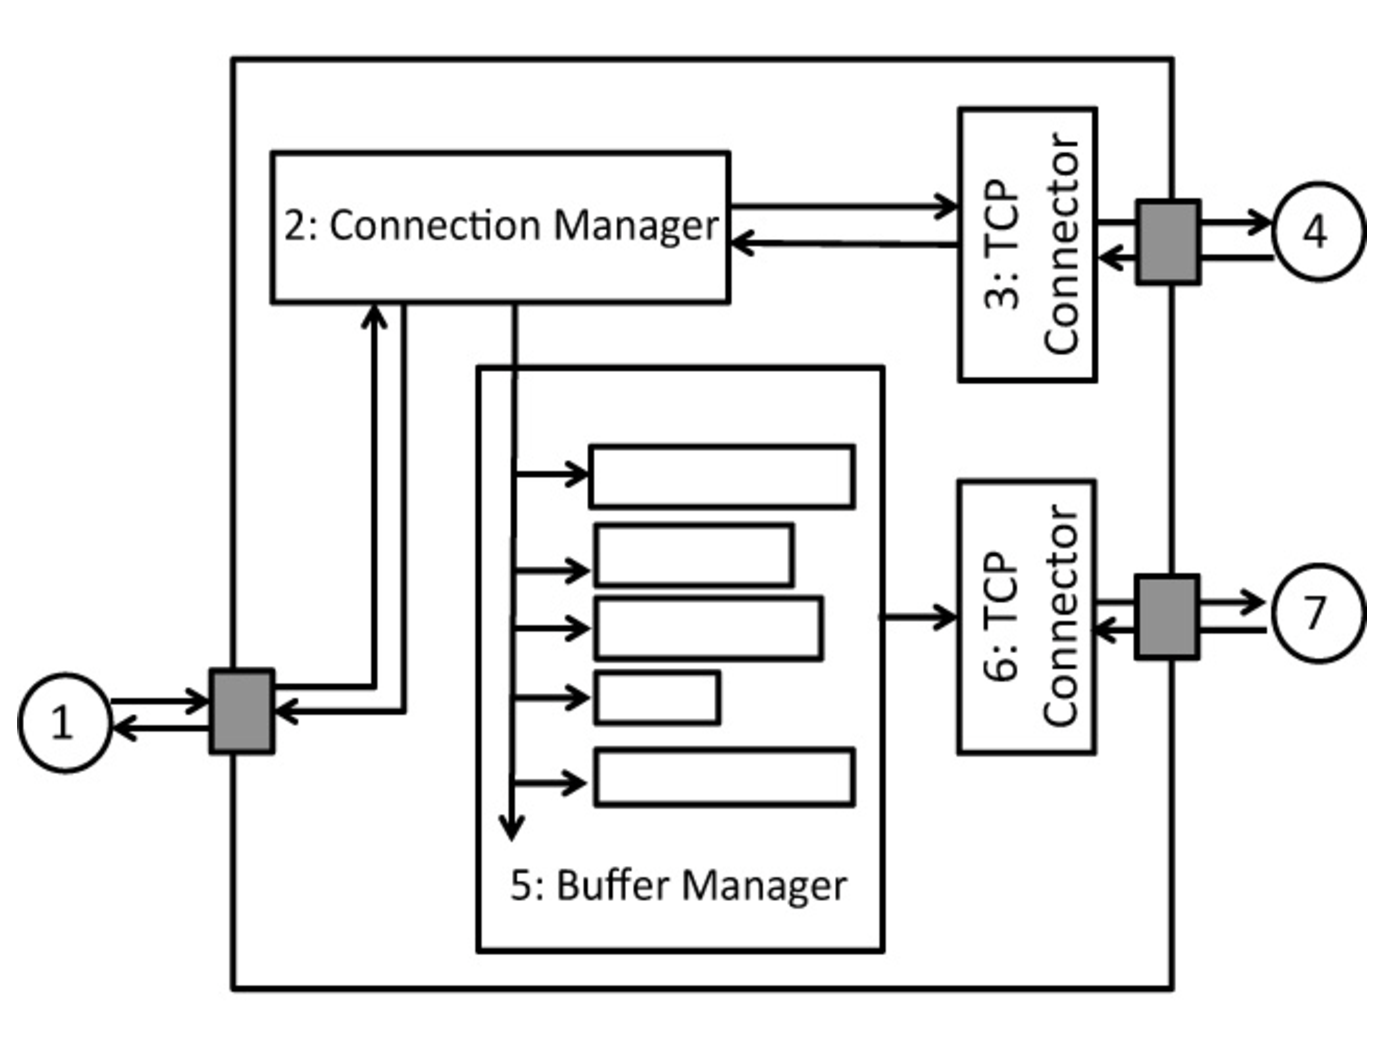
\includegraphics[width=0.4\textwidth]{figs/duplicator.eps}
    \caption{Description of the Network Duplicator}
    \label{fig:duplicator}
  \end{center}
\end{figure}

The workflow of each component is as follows: Traffic from the client (Node 1 in figure \ref{fig:duplicator}) is forwarded to the Connection Manager(Node 2 in figure \ref{fig:duplicator}). 
The connection manager essentially is a socket reader which copies, parses the incoming traffic. 
Based on the type of TCP request, a new connection is created or data is forwarded/received to/from the TCP Connector( Node 3, figure \ref{fig:duplicator}) which in turn creates a connection to actual production server.
In this way the connection manager and TCP connector follow the TCP state machine hence mantaining network packet sanity while forwarding traffic to the production container.
Simultaneously, the connection manager creates an internal copy of incoming traffic, and parses and sends it to the Buffer Manager (Node 5, figure \ref{fig:duplicator}).
In a naive scenario the connection could be simply forwarded to the test-container, and the traffic would be managed by itself. 
However, it is likely that the rate of traffic consumption by the test-container is less than the production container. 
This gives us several startegies to design the duplication of traffic to the test container:

\begin{enumerate}

  \item \textbf{Synchronized}

  A naive startegy is to send TCP requests to the production node, and then send it to the request node

  \item \textbf{Asynchronous}

Launch two threads on accepting each TCP request. For each session of TCP requests, two threads manage sending and receiving  to the production and test-container

  \item \textbf{Synchronized Partial Order Multi-Threaded Queue}

Launch two threads, track slowdown of the duplication thread.

  \item \textbf{Multi-Duplication}

Launch multiple duplication threads

\end{enumerate}

Since the speed of input from the client is not in sync production-container, we need to buffer incoming traffic and relay it to the the TCP Connector(Node 6, figure \ref{fig:duplicator}) as soon as the test-container is ready for new traffic. 
Since parallel connections can be initiated by the client on the same TCP port, the BufferManager creates multiple buffers for each connection, and initiates new connections by following the same causal flow of the packets received from the client. 
Unlike record-replay systems \textit{Parikshan} does not claim to have strong consistency requirements, and does not need to exactly follow the production container as the goal is not reproduce all non-determinism in the production environment, but instead capture input non-determinism, and complete system state from a given point of time.
We discuss consistency requirements further in section \ref{sec:consistency}

\subsubsection{Time Delay and Buffer Management}
\label{sec:TimeManagement}

%It is possible that in heavy load conditions the buffers in the Buffer Manager may overflow. 
%Depending on the use-case the BufferManager can then trigger the CloneManager, which closes the analysis time-window and launches a fresh clone.
Incoming traffic may potentially have a cumulative effect which will eventually lead to a buffer overflow in the BufferManager, hence leading to packet drops. 
This behavior is similar to packet dropping in classical TCP buffers, which rely on retransmission of incoming packets from the client.
However in our case if packets are dropped the client cannot retransmit them as it not in sync with the test container.
Hence in some cases \textit{Parikshan} analysis, has to be restricted to a time-window dependent on the load of incoming traffic and the slowdown experienced by the test-container.

%Let the rate of incoming traffic be \lambda

\subsection{Network State Model}
\label{sec:networkStateModel}

Network communication in most applications consists of two core types of protocols: UDP \& TCP.
The UDP(User Datagram Protocol) allows the applications to send messages(referred to as datagrams) to other hosts in the network without prior communications to set up any transmission channels.
UDP uses a simple communication mechanism while minimizing protocls. 
It has no handshaking dialogues or acknowledgement of package delivery. It is broadly used for network traffic where speed is much more important than reliability (viz. network streaming applications like video etc.)
On the other hand TCP(Transmission Control Protocol) is a reliable error checked delivery stream.
It involves initially establishing the connection, and allowing for packet re-delivery or re-ordering to allow for reliable and dependable connection. 
While TCP is slower than UDP it is preferred for most normal connections between clients and server applications.

Since the UDP protocol has no error management mechanism, it automatically follows that machine state in a UDP connection is not important.
Hence in our design the duplicator can easily flood packets to the cloned UDP server by simply sending packets to the targeted host and port. 
Our solution for this is 


\section{Implementation}
\label{sec:implementation}

\parikshan is built on top of a production user-space container virtualization software, OpenVZ \cite{openvz}, with Centos 6.5 with Linux Kernel 2.6.32.
Each container layout is managed using PLOOP\cite{ploop} devices to enable faster and easier cloning.
The OpenVZ functionality, was extended to enable live-cloning as explained in section\ref{sec:design}.
We modified and used the OpenVZ toolkit vzctl version 4.7 to create our cloning, creation and destroy scripts for the container. 
While the technology has also been tested on Debian systems, the evaluation in this paper has been done on RHEL(Centos) Systems. 
%For our evaluation, we have not put in resource restriction on the containers (i.e. the containers have access to the same hardware resources as the host machine).
%Users using \parikshan may put resource restriction as required.
%\parikshan also requires a number of commonly available linux modules to allow for network connectivity and 

We have tested the system in 3 different configurations. 
In the first case we tested \parikshan 's internal mode configuration by installing \parikshan in a single host OS, with Intel Core 7 CPU, 8 Cores, 16GB RAM, and running Ubuntu 14.04. 
\parikshan was installed on multiple VM's running on the host OS using KVM based virtualization. 
Containers were cloned across these machines, with a seperate VM acting as the client.
We used NAT, and ip namespaces for network access to the VM's.

In the second mode, we tested our system's external mode by installing \parikshan on the base kernel in identical host nodes. 
Each of these host nodes have an Intel Core 2 Duo Processor, 8GB of RAM, and ran Centos 6.5 with Linux Kernel 2.6.32.

In the third mode, we tested our system on Google's Cloud Infrastructure (Google Compute \cite{gcompute}).
The production and the test container's were run on different virtual nodes, with 2 VCPU's and 4G RAM. 
The main advantage of using the Google Compute Engine was to run our cloning scripts on real data-centers, and also to scale out our evaluation. 

The network proxy was implemented in C/C++.
The forwarding in the proxy is done by forking off multiple processes each handling one send/or receive connection in a loop.
Data from processes handling communication with the production container, is  transferred to those handling communication with the test containers using pipes. 
%\noindent\section{Inserting probes \& Performance Analysis}
\label{sec:trigger}

The key idea behind sandbox testing is to debug problems in real-world scenarios
Once we have forked off a clone, we are now ready to do some deeper analysis. 
Here we explain how debugging can potentially be done in real live systems to give the operator and developers a deeper view of the target application.
\parikshan could potentially be used in several ways for application debugging and introspection. 
However, in the interest of brevity, we talk about only two categories. 
Firstly, inserting probes which can help in generating traces so that the user can understand the execution path of the application.
Secondly, performance analysis, such as memory usage, number of context switches etc. this can give the user an idea of what could be the bottleneck for the target application.

%By design, \textit{Parikshan} can allow a variety of test cases. 
%We divide such analysis in two parts based on the time window required for analysis: (1).Statistical

\noindent\subsection{Inserting Probes \& TestCases}
\label{sec:unitTests}

Execution tracing is a key debugging tool for locating any bugs. 
Essentially, an execution trace is a log of the functions executed, values of certain variables being tracked etc. within a time-frame.
The path taken and the value of the variables are important as they explain the logic flow of the application for the \emph{"configuration"} and \emph{"context"} at the time of creating the clone.
To generate this trace, we insert probes or watch points for variables in the application similar to existing development phase debugging tools such as GDB(gnu debugger) \cite{gdb}.
Inserting probes in the sandbox can be done using any existing dynamic instrumentation tools  such as PIN \cite{pin}, Valgrind \cite{valgrind}, Dyninst \cite{dyninst}.
For our purposes we used \iprobe\footnote{we have used iProbe only because of our familiarity} \cite{iProbe} a dynamic binary instrumentation tool designed by the authors to insert probes in running applications. 
 \iprobe  uses compile time flags to generate placeholders in the binary, and inserts instrumentation probes in the binary at run-time.
Users can use it to insert print statements on function executions. 



\subsection{Performance Analysis}
\label{sec:Performance}

While execution traces provide a good indication for localizing bugs, often system level statistics, such as memory usage, cpu usage, context switches, number of threads can be a good indication towards bug localization.
This is especially true if the bug is because of a configuration error or in the interaction of the application to the base kernel system.

Given that the production and the test-container have similar resources allocated to them, we believe that the system level statistics of the test-container will be a close representation of the original as it was a clone of the production container.
We accept that it cannot represent the production container entirely, as there is bound to be some non-determinism in the containers.
However, any input driven state changes are bound to be caught.

Previous approaches including some of the work done by the authors \cite{clue} \cite{kscope} and others in academia \cite{sherlog} \cite{vscope} have often used kernel level statistics or system call traces, in localizing bugs. 
The idea behind these approaches is generally to provide a black-box solution to applications.
However, in practice they can only be used in lower workload's or can only provide vague clues as they need to restrict the amount of instrumentation to avoid a heavy overhead.

%Analysis which need a long time window to record, and run the status across multiple requests are considered as long running analysis. 
%Such analysis can be considered to be similar to monitoring of live applications, and are usually statistical in nature.
%Typically tools such as PIN \cite{pin}, Valgrind \cite{valgrind}, Dyninst \cite{dyninst}, can do deep analysis without modifying the logic of the application.
%However, they impose a heavy penalty in terms of performance.
%Such tools can be easily used in \textit{Parikshan}, without effecting system performance.
%However, there are a few challanges with such statistics which need a longer window to run.


%\section{Network Issues}
\label{sec:network_issues}

There are several problems that can effect the execution of sandbox testing. 

\begin{itemize}
  \item \textbf{Stateful Connections}
  \item \textbf{Time Lag}
\end{itemize}

\section{Case Studies}
\label{sec:casestudy}

\begin{table*}[ht!]
\centering
\begin{tabular}{|c|c|c|c|c|c|c|c|}
\hline
\begin{tabular}[c]{@{}c@{}}\textbf{Bug} \\ \textbf{Type}\end{tabular}                        & \textbf{Bug Desc}                                                       & \textbf{Application}           & \begin{tabular}[c]{@{}c@{}}\textbf{Tool} \\ \textbf{Used}\end{tabular}       & \begin{tabular}[c]{@{}c@{}}\textbf{Debug} \\ \textbf{Mechanism}\end{tabular} & \begin{tabular}[c]{@{}c@{}}\textbf{Slow-}\\ \textbf{down}\end{tabular} & \begin{tabular}[c]{@{}c@{}}\textbf{Nodes}\\ \textbf{Cloned}\end{tabular} & \begin{tabular}[c]{@{}c@{}}\textbf{Comments/}\\ \textbf{Bug Caught}\end{tabular} \\ \hline
\multirow{3}{*}{\begin{tabular}[c]{@{}c@{}}\textbf{Performance}\\ \textbf{Bug}\end{tabular}} & \#15811                                                        & MySQL                 & iProbe                                                     & Exec. Trace                                                & 1.5x                                                 & 1                                                      & Yes                                                            \\ \cline{2-8} 
                                                                           & \#45464                                                        & Apache                & iProbe                                                     & Exec. Trace                                                & 1.4x                                                 & 1                                                      & Yes                                                            \\ \cline{2-8} 
                                                                           & \#49491                                                        & MySQL                 & iProbe                                                     & Exec. Trace                                                & 1.8x                                                 & 1                                                      & Yes                                                            \\ \hline
\multirow{2}{*}{\begin{tabular}[c]{@{}c@{}}\textbf{Memory} \\ \textbf{Leak}\end{tabular}}    & Injected                                                       & Glassfish             & \begin{tabular}[c]{@{}c@{}}VisualVM/\\ mTrace\end{tabular} & \begin{tabular}[c]{@{}c@{}}Memory\\ Profiling\end{tabular} & 3x                                                   & 1                                                      & Yes                                                            \\ \cline{2-8} 
                                                                           & Injected                                                       & MySQL                 & Valgrind                                                   & memcheck                                                   & N.A                                                   & 1                                                      & \begin{tabular}[c]{@{}c@{}}Yes, with\\ overflows\end{tabular}  \\ \hline
\multirow{2}{*}{\begin{tabular}[c]{@{}c@{}}\textbf{Config.} \\ \textbf{Errors}\end{tabular}} & DNS                                                            & JBOSS                 & DTrace                                                     & Tracing                                                    & 1.3-4x                                               & 2                                                      & Yes                                                            \\ \cline{2-8} 
                                                                           & \begin{tabular}[c]{@{}c@{}}Max no. \\ of threads\end{tabular}  & MySQL                 & DTrace                                                     & Tracing                                                    & 1.5x                                                 & 2                                                      & Yes                                                            \\ \hline
%\multirow{2}{*}{\begin{tabular}[c]{@{}c@{}}Concurren \\ Bug\end{tabular}}  & \begin{tabular}[c]{@{}c@{}}Atomicity \\ Violation\end{tabular} & Apache                &                                                            &                                                            &                                                      &                                                        & Maybe                                                          \\ \cline{2-8} 
%                                                                           & \begin{tabular}[c]{@{}c@{}}Race\\ Condition\end{tabular}       & Apache                &                                                            &                                                            &                                                      &                                                        & Maybe                                                          \\ \hline
%\multirow{2}{*}{\begin{tabular}[c]{@{}c@{}}Crash \\ Bugs\end{tabular}}     & Server Crash                                                   & Apache                & N.A                                                        & N.A                                                        &                                                      &                                                        & Cannot Debug                                                   \\ \cline{2-8} 
%                                                                           & Request Crash                                                  & \multicolumn{1}{l|}{} & \multicolumn{1}{l|}{}                                      & \multicolumn{1}{l|}{}                                      & \multicolumn{1}{l|}{}                                & \multicolumn{1}{l|}{}                                  & Yes                                                            \\ \hline
\end{tabular}\caption{Case-Study of production system bugs, with approximate slowdowns, debug mechanisms, and tools used.}
\label{table:casestudy}
\end{table*}

%Here we show how \parikshan can be applied to some real-life bugs.
%Table \ref{table:casestudy} shows several bugs which we debugged using \parikshan, and the various techniques we used to localize the bug.
%Parikshan enables the users to freely run any test-case in the test-container while not effecting the production container. 
%At the same time the output of these tests should not effect the functionality or the performance of the production system.
%The main advantage of such a system can be seen in service oriented applications which are user facing and can hence ill-afford to be shutdown for inspecting bugs.
%As mentioned earlier, another major advantage is that we are able to capture live user-input. \\

%\subsection{Debug Tools and Mechanisms}
%\label{sec:debugMechanisms}

Production applications are usually deployed with transaction logs, and error logs that alert the operator of any anomalous behavior.
%Often the information in such logs is insufficient to find the root-cause, and can give false-positives or skip errors altogether.
Debuggers use these logs, to run offline test-cases in order to find the root-cause of any bugs. 
This process may need multiple iterations between the operator and developer, as more information may be required from the production system. This eventually increases the time to debug the error.
%Since only minimal dynamic instrumentation is allowed, developers go through a trial and error process of increasing the coverage of instrumentation 
%(or have higher instrumentation with the production service suffering an overhead).

%In this section we briefly mention various debug mechanisms, and what they generally involve. 
%We discuss how they can be successfully applied to bug cases we found in production systems in the next subsection.
The idea behind \parikshan is to allow operators to use debugging tools and mechanisms in the production environment, that one would normally use in the development environment.
These tools allow developers to better understand program flow and data flow, which is key to localizing the root cause of any bug.
Dynamic instrumentation tools like DTrace~\cite{dtrace}, and iProbe~\cite{iProbe} can generate \emph{execution traces}, which give insight into the program flow (functions, and conditional statements executed).
iProbe has statically compiled ``hooks'' in the beginning and end of functions in the target applications, which can be patched with dynamic instrumentation on-the-fly.
On the other hand, DTrace uses interrupt mechanisms to insert a probe at any point in the application using symbolic information. 
%Data flow on the other hand requires much finer instrumentation. 
Similarly, tools like dyninst~\cite{dyninst} allow users to track data-flow of variables in the code.
\emph{Memory profiling} tools like Valgrind~\cite{valgrind}, PIN~\cite{pin}, and VisualVM~\cite{visualvm} give insight into memory allocation and deallocation, thus helping in catching memory leaks.
%Another tool, Valgrind~\cite{valgrind} can do systematic checking of memory allocation, but has a high overhead and requires application restart.
%On the other hand, profiling tools like VisualVM~\cite{visualvm}, and PIN~\cite{pin} can be dynamically attached to track memory usage. 
%The downside to this is that it halts progress in the application, unlike execution trace which imposes a slowdown. 
%Other mechanisms such as \textbf{delta-debugging}, and \textbf{heap-dump} allow users to modify variables to check if that resolves problems hence changing it's behavior.
Next, we discuss how these techniques can be applied to different categories of real-life bugs with the help of the \parikshan framework:

%\subsection{Bug Categories}
%\label{sec:bugCategories}

%\subsubsection{Performance Bugs}
%\label{sec:performanceBugs}
\noindent
\textbf{Performance Bugs}: One of the most subtle problems that manifest in production systems is performance bugs.
% especially in usecases which were earlier not thought of during stress testing.
These bugs do not usually lead to crashes, but cause significant impact to user satisfaction.
%The problem can manifest itself because of some configuration parameter, or redundant function calls, non-optimal path, and can require either a bug-fix, or a new feature addition.
A casestudy~\cite{shanluPerf} showed that a large percentage of real-world performance bugs can be attributed to uncoordinated functions, executing functions that can be skipped, and inefficient synchronization among threads (for example locks held for too long etc.).
Typically, such bugs can be caught by function level execution tracing and tracking the time taken in each execution function.
Another key insight provided in~\cite{shanluPerf} was that two-thirds of the bugs manifested themselves when special input conditions were met, or execution was done at scale. 
Hence, it is difficult to capture these bugs with traditional offline white-box testing mechanisms.

%\noindent
In an empirical evaluation of three such real-world bugs, we used \parikshan and iProbe~\cite{iProbe} (a dynamic instrumentation tool) to capture a representative function trace.
The tracing caused a 1.5x - 2x slowdown in the targeted session of the application,  with no impact on the production system.
For one of the bugs in  MySQL (Bug 15811), it was reported that some of the user requests which were dealing with complex scripts (Chinese, Japanese), were running significantly slower than others.
To evaluate \parikshan, we re-created a two-tier client-server setup with the server (container) running a buggy MySQL server. 
We generated a random workload of user-requests, including queries that triggered the bug.
Now the slow queries may be reported by either a user, or a transaction latency monitoring available in several production systems. 
Based on this trigger, we created a live clone of the MySQL container. 
We then inserted function level instrumentation in MySQL for higher level functions, object constructors, and destructors belonging to each module in the code.
Finally, we used the query handler to trigger instrumentation for queries containing complex scripts(this ensures no slow-down for other queries).
%For all transactions with insert queries with a complex character set, we triggered instrumentation to track execution in high granularity functions in insert and character\/string module.
We then compared the profile (time taken in each function) of the queries for complex scripts, with the queries for Latin scripts.
Using trial-and-error, and iteratively digging into deeper functions, we were able to localize the bug to string compare functions in MySQL.
%Using the profile for regular latin charactersets, and comparing it to complex charactersets (chinese, japenese) we were easily able to localize the bug to the compare functions in the string module.
%Using a trial and error method we profiled high granularity functions in MySQL and gradually looked at finer granularity modules to isolate the performance problem.
%This allowed us to successfully isolate the function with the performance problem.
%The MySQL queries, were only a few KB's so we were able to queue up several requests in the pipe and there was no divergence in the output produced by both the debug container and the production container. 


%\subsubsection{Memory Leaks}
%\label{sec:memoryLeaks}
\noindent
\textbf{Memory Leaks}: %Localizing a memory leak takes us further than simply execution tracing. 
Memory leaks are a common error in service oriented systems, especially in C/C++ based applications which allows low-level memory management by users.
These leaks build up over time, and can cause slowdowns because of resource shortage, or crash the system.
Debugging leaks can be done either using systematic debugging tools like Valgrind, which use shadow memory to track all objects, or memory profiling tools like VisualVM, mTrace, or PIN, which track allocations, de-allocations, and heap size.
Although valgrind is more complete, it has a very high overhead, and needs to capture the execution from the beginning to the end (i.e., needs application restart).
On the other hand, profiling tools are much lighter, and can be dynamically patched to a running process.

For our empirical evaluation, we injected repetitive memory allocations to an object in a glassfish app-server, and sent requests to app-server to trigger these allocations.
We then, used \parikshan to clone \& create a debug-container, where we used VisualVM to track the increase of heap-size, and object allocations.
Tracking memory allocation allowed us to localize the class file causing the memory leak, which greatly simplifies finding the root-cause.
We experienced a slowdown of 3x, but did not observe any overflow in the buffer.

We also used memory leak detection using Valgrind in MySQL for an injected memory leak in the request handler for MySQL.
We wish to stress here, that while tools like valgrind, need application restart, and will most likely cause extremely high slow-downs in the debug-container, \parikshan can still be helpful, as it can debug a small part of the target system in isolation, thereby quickly resolving errors.
Application service restart may not lose context in all applications, especially a database application has a persistent database, and may exhibit errors even after the restart.
With Valgrind, we saw requests being dropped in the proxy because of the high overhead, but we were able to capture and trace memory leaks for several requests.


\iffalse
Memory leak analysis can be done by doing memory allocation function profiling (malloc, free etc.) or using tools like Valgrind~\cite{valgrind}, which use shadow memory techniques to trace all actively allocated objects.
While shadow-memory tools are good for development debugging, it cannot be applied to real-production environments as they cannot be dynamically attached to a running service, and the process needs to be closed to compute which objects remained allocated or to show dangling reference (actively allocated memory may or may not be used in the future) etc.. Additionally these tools are resource hungry and have a high overhead (~4-6X).

In our memory leak case study, we first profiled the application to find transactions that could potentially be the cause of the memory leak. 
We then filter out everything except the suspect transactions, and restart mysqld service with valgrind memcheck tool turned on.
The valgrind tool was able to summarize and point to the root-cause of the bug which we validated from the bug report.
In this case the considerable overhead because of valgrind, and the fact that it serialized the execution (other transactions were not able to follow), led to transactions being dropped in the proxy. 
However, this did not impact us in finding the root cause.

%\noindent
In another memory leak scenario for Java Glassfish~\cite{glassfish} app server, we were able to apply a memory profiler (visualVM), to look at allocation and deallocation patterns.
This has comparatively lesser overhead, and can point to stale objects, or can profile how different classes are using the heap memory.
%In cases where memory leak exhibits because of the application state after a long running execution, memory profiling may be a better choice than shadow memory tools, as they require a service restart.
Using memory profiling in \parikshan will allow users to capture the ``long-running'' context of the application which may be important to capture the bug.
\fi

\noindent
\textbf{Configuration Errors}:
Configuration errors are usually caused by wrongly configured configuration parameters, i.e., they are not a bugs in the application, but bugs in the input (configuration).
Configuration bugs usually get triggered at scale, or for certain edge cases, making them extremely difficult to catch.

For our empirical evaluation, we created a 3 tier (Apache, JBoss, MySQL) service using Java PetStore~\cite{petstore} a J2EE example application.
We inserted a configuration error by setting an arbitrarily low number for the max. number of requests MySQL can handle.
We then triggered requests to PetStore, and found some of them timing out.
Using \parikshan, we cloned both JBoss and MySQL servers, to captured the flow of queries across distributed machines.
We traced higher object constructors, and library calls to track the execution.
This allowed us to see that the MySQL server was not creating worker threads for the incoming requests(no calls to libc fork events).
Debug logs had been turned off for optimization, hence the error could not be easily reported. 
\parikshan was able to successfully localize the error to mis-configuration in the ``maximum no. of worker thread'' allowed parameter.
While the error may seem simple, without \parikshan an offline testbed would be required with a large enough test workload.


% it was reported that certain queries were returning empty or ``null'' pages. 
%The operator can potentially find out which machines in the cluster were affected by this bug.
%Since debug logs have not been turned on we can only see the path the query is taking but do not see any error report generated.
%This can be used by the operator, to find which containers need to be cloned. 

%\subsubsection{Configuration Bugs}
%\label{sec:configurationBugs}

%\subsubsection{Concurrency Bugs}
%\label{sec:concurrencyBugs}

%\textbf{Concurrency Bugs}: Concurrency bugs are caused because of non-deterministic execution in multi-threaded applications.
%These bugs are particularly difficult to catch in white-box debugging as 

%\subsubsection{Integration Bugs}
%\label{sec:integrationBugs}
%\subsection{Debugging Techniques}
%\label{sec:debugTechniques}
%\par \noindent
%\subsection {CaseStudy 2: Performance Profiling, using dyninst}
%Demand Driven Testing - https://www.cs.virginia.edu/~soffa/Soffa_Pubs_all/Conferences/Demand-driven.Misurda.2005.pdf
%@Nipun- I don't think either of the next two make a lot of sense
%\par \noindent \textbf{CaseStudy 3: A/B Testing}
%A/B Testing 
%http://www.polteq.com/wp-content/uploads/2013/02/testingexperience20_12_12_Marc_van_t_Veer.pdf
%\par \noindent \textbf{CaseStudy 4: Fault Tolerance Testing}
%Fault Injection to look at fault tolerance
%Fault Injection in netflix http://techblog.netflix.com/2012/07/chaos-monkey-released-into-wild.html
%Security Honeypots? 
\iffalse
%\par \noindent
\subsection{Case-Study 1: Debugging using Execution Tracing of MySQL bug 18511}  
Performance profiling such as function execution trace, execution time, resource usage etc., is often used to indicate and localize performance bugs in real world systems. 
While performance profiling is simple to implement, it obviously incurs an overhead and will effect user-experience of the target system.
Effectively, this means that despite it's advantages, the amount of profiling that can be done in a production system is extremely limited. 

As our first case study we focused on profiling and capturing a performance bug in a session with several randomly created user transactions to MySQL. 
It was reported by users, that some of the user requests were running significantly slower than others.
To test out \parikshan to catch this bug, we re-created a 2 tier client-server setup with the server(container) running a buggy mysql server application, and made a random workload with several repetitive instances of queries triggering the bug.
We initiated debugging by creating a live clone of the container running the mysql server.
Using a trial and error method we profiled high granularity functions in mysql and gradually looked at finer granularity modules to isolate the performance problem.
This allowed us to successfully isolate the function with the performance problem.

We believe this case study shows a classical performance bug, where \parikshan can be used.
Firstly, it's a performance bug which is non-critical i.e. does not lead to crashes etc.
\parikshan has been designed to look into real live bug diagnosis, rather than looking at bugs after a crash etc.
\footnote{A lot of SOA applications are fault tolerant, and can continue even after the crash by relaunching processes etc. Potentially \parikshan can also be used in such a scenario to trace the crash itself.}
Secondly, we assume that the user-input (which caused the bug), occurs fairly frequently.
In this case, a database query which looks into data containing chinese characters, or japanese characters could be a fairly common occurence.
In our experience we found several such performance bugs which occur in only a small percentage of user transactions.
These bugs are often difficult to catch as they happen only in corner case inputs, and generally do not lead to application crashes.
\parikshan would be useful to debug such performance errors, by giving deep insight in a live running system.
\fi


\section{Evaluation}
\label{sec:evaluation}
In this section we present the evaluation of Parikshan. 
The key questions facing us were:
\begin{itemize}
%  \item How can \parikshan be used in the real world? 
%  \item Does the test container faithfully represent the execution and the state of the production container? 
   \item How does cloning the container effect the performance of the production container?
   \item How does running tests in the test-container effect the performance of the production container?
   \item How long of a testing-window do we have? 
\end{itemize}

In order to answer these questions, we seperated our evaluation in looking at two different stages: cloning stage, time-window analysis.

\subsection{Cloning: Micro-Benchmarks}
\label{sec:performance}

\begin{table*}[ht]
  \centering
    \begin{tabular}{ | p{4cm} | l | l | l | l | l | l | l | l | l |}
    \hline
    \textbf{Modes} & \multicolumn{3}{|c|}{\textbf{Internal Mode}} & \multicolumn{3}{|c|}{\textbf{External Mode}} & \multicolumn{3}{|c|}{\textbf{Google Compute}}\\\hline
    \textbf{ } & \textbf{Cl} & \textbf{Hog} & \textbf{Hog+Cl} & \textbf{Cl} & \textbf{Hog} & \textbf{Hog+Cl} & \textbf{Cl} & \textbf{Hog} & \textbf{Hog+Cl} \\ \hline
    \hline
    \textbf{Throughput} & -- & 1691.0 req/s & 1509 req/s & -- & 712 & 625 & -- & 510 & 450\\ \hline
    \hline
    \textbf{Suspend + Dump} & 0.49 & -- & 0.46 & 0.00 & 0.00 & 0.00 & 0.00 & 0.00 & 0.00\\ \hline
    \textbf{Pcopy after suspend} & 0.22 & -- & 0.27 & 0.00 & 0.00 & 0.00 & 0.00 & 0.00 & 0.00\\ \hline
    \textbf{Copy Dump File} & 0.62 &  -- & 0.64 & 0.74 & 0.59 & 0.65 & 0.00 & 0.00 & 0.00\\ \hline
    \textbf{Undump and Resume} & 1.33 &  -- & 1.53 & 0.74 & 0.59 & 0.65 & 0.00 & 0.00 & 0.00\\ \hline 
    %\textbf{--------------} & --- & --- & --- & --- & --- & --- & --- & --- & --- \\ 
    \hline
    \textbf{Total Suspend Time} & 2.66 &  -- & 2.91 & 0.74 & 0.59 & 0.65 & 0.00 & 0.00 & 0.00\\ \hline
    \end{tabular}
\caption{Performance of Live Cloning (external mode) with a random file dump process running in the container}
\label{table:clonePerf}
\end{table*}

The profile of the cloning operation can be divided in 4 stages: 
(1) Suspend \& Dump: this is the time taken to suspend the container, 
(2) Pcopy after suspend: which does the rsync after the suspend of the file system of the container, 
(3) Copy Dump File: which copies the process state, and finally 
(4) Undump and Resume: which is the time taken to resume the containers. 
We first looked at the performance of the cloning operation to look at the time taken to do cloning while. 
In table \ref {table:clonePerf}, we show the suspend times in all 3 modes: internal, external, and google-compute, while comparing it with a production container, that is idle vs. a container which is running an apache hog benchmark \cite{httperf} on it. 
The first column gives the average performance of the cloning operation without any hog operation running on it.  
An idle or a containter with minimal processing is cloned relatively fast ~ 2.66 seconds on the idle container. 
We then tried to run an apache hog to make a baseline of apache's performance without cloning, and found that a simple page fetch gave us a throughput of 1691 req/s (internal mode), and then we tried to do cloning of the same container while running the hog. and found negligible change in the cloning performance.
The key idea behind this performance 

As explained earlier, the cloning process can be divided into two parts: an rsync operation which does an ``pre-copy'' of the VM, and a followup rsync operation while the target container is suspended, to make sure that both the production and test containers have the exact same state.
The idea is to reduce the time taken to suspend the production container, so that it has minimal effect on the user.
The main factor that effects this is the number of ``dirty pages'' in the suspend phase, which have not copied over in the pre-commit rsync operation.
Natrually, the number of write operations in the container while cloning the container, will increase the number of dirty pages, and increase the time of the suspend operation.



\vspace{-2mm}
\section{Applications of Live Debugging}
\label{sec:application}
The concept of debugging typically encompasses more than just localizing the bug, but also includes attempted fixes, tests of those fixes, and patching. Here, we briefly discuss here how existing techniques can be directly applied in \parikshan. 
Further details about this can be found in our tech-report~\cite{parikshanTR}

\noindent
\textbf{Statistical Testing:}
One well known technique for debugging production applications is statistical testing. 
This is achieved by having predicate profiles from both successful and failing runs of a program and applying statistical techniques to pinpoint the cause of the failure.
The core advantage of statistical testing is that the sampling frequency of the instrumentation can be decreased to reduce the instrumentation overhead.
Despite it's advantages the instrumentation frequency for such testing to be successful needs to be statistically significant. 
However overhead concerns in the production environment limit the frequency of instrumentation.
In \parikshan, the buffer utilization can be used to control the frequency of such statistical instrumentation in the debug-container. 
This would allow the user to utilize the slack available in the debug-container for instrumentation to it's maximum, without leading to an overflow. 
Thereby improving the efficiency of statistical testing.

\noindent
\textbf{Record and Replay:}
%Error logs in applications, or monitoring tools~\cite{clue,magpie,dtrace}, can be used to do light-weight anomaly detection in production systems.
%However, these techniques are usually insufficient to capture the context of the bug.
Record and Replay techniques have been proposed to replay production site bugs. 
However, they are not yet used in practice as the overhead they can impose unacceptable overheads in the service processing times.
\parikshan debug containers can be used to do recording as long as the overhead does not lead to buffer overflows.

\noindent
\textbf{Distributed Debugging:}  
Large scale distributed systems are often comprised of several interacting services such as storage, NTP, backup services, controllers and resource managers.
\parikshan can be used on one or more containers, and can be used to clone more than one communicating service.
Based on the nature of the service, it may be (a). Cloned, (b). Turned off or (c). Allowed without any modification.
For example, storage services supporting a ``debug-container'' need to be cloned or turned off (depending on debugging environment) as they would propagate changes from the debug container to the production containers.
Similarly, services such as NTP service can be allowed to continue without any cloning as they are publish\/subscribe broadcast based systems and the debug container cannot impact it in anyway.
Furthermore, instrumentation inserted in the debug-container, will not necessarily slowdown all services.
For instance, instrumentation in a MySQL query handler will not slowdown file-sharing or NTP services running in the same container.

\noindent
\textbf{Patch Testing:}
Bug fixes and patches to resolve errors, often need to undergo testing in the offline environment, and are not guaranteed to perform correctly.
Patches can be made to the debug-container instead. 
The fix can be traced and observed if it is correctly working, before moving it to the production container.
\section{Discussion}
\label{sec:discussion}

Designing large scale distributed systems is complex. They are often comprised of several interacting services such as storage, ntp, backup service, controllers and resource managers.
Based on the design and architecture of the system, services for the cloned ``debug container'' may need to be (a). Cloned, (b). Turned off or (c). allowed without any modification.
For example, storage services supporting a ``debug-container'' need to be cloned or turned off(depending on debugging environment) as they would propogate changes from the cloned container to the production containers.
Similarly, services such as ntp service can be allowed, as they are publish\/subscribe systems and the debug container cannot impact it in anyway.
\parikshan can be used on one or more containers, and can be used to stub out more than one communicating service depending on the system requirement.
%In this paper we have shown a proof-of-concept design and implementation with several case studies on  how \Parikshan can be applied for real-world debugging.

%\textbf{Concurrency non-determinism}: \parikshan can capture the system state and the user input.
%However, it is still possible that we will miss errors which happen because of specific schedules or caching in the production system.
%\parikshan can still be applied 

%\subsection{Rate Limiting}
%\label{sec:ratelimiting}

%\textbf{Rate Limiting}: As we show in section \ref{sec:evaluation}, at extremely high write I/O's it is possible that the suspend time for cloning is sometimes prohibitively high, and can cause TCP timeouts. 
%The operator can thereby chose to use cloning and sandboxing, at low workload conditions. 
%Alternatively, a simple solution to this problem is to use rate-limiting at the proxy which would allow the I/O consumption in the target container to become lower, thereby reducing the suspend time.
%Rate limiting is a commonly used mechanism in proxies, while it reduces the QoS of the application momentarily, it may be better for fast bug resolution.

%\subsection{Dynamic Proxy Insertion}
%\label{sec:dynamicProxyInsertion}

%\textbf{Dynamic Proxy Insertion}: While cloning does happen live, we do not really need to have the proxy to be inserted dynamically as well. 
%Proxies are commonly used in several applications so they can be essentially all the time. 
%However, based on design choice, the proxy can be inserted by starting it up on any server, and then putting a flow redirection rule in the router using dynamic network programming mechanism such as OpenFlow\cite{openflow}.
%Router flows are updated dynamically, and are \texttt{flow-based}, hence can be redirected on the fly using an openflow\cite{openflow} controller.

%\subsection{Slowdown}
%\label{sec:slowdown}


%\subsection{Consistency Requirements}
%\label{sec:consistency}
\iffalse

\textbf{Consistency Requirements}: Not all debugging may require very high consistency requirements, and not all overflows would mean that the clone is suddenly out of sync.
In such cases the time-window can be arbitrarily long. 
For example in mysql read transactions, even if there is a transaction failiure or an overflow, it will not effect MySQL itself.
Even with an overflow in some write operations, we could get a weakly consistent representation of the production system's execution.


\subsection{Non-Determinism}
\label{sec:nonDeterminism}

Execution of the same input in different conditions can produce different outputs from an application, this behavior is referred to as non-deterministic execution.
With the exception of dedicated controlled executions in embedded systems etc., most large scale applications and complex systems exhibit non-determinism, which is what makes debugging a challenge.
Broadly non-determinism can be caused because of the following reasons: 1. Input non-determinism, 2. Configuration non-determinism, 3. Concurrency based non-determinism.

Input non-determinism is non-deterministic behavior caused because of different input received by the application (eg. requests to the server, user input etc.). 
Obviously, any output in the application and it's execution trace, will depend on the input it receives. 
In offline debugging it is often difficult to capture all possible inputs, and hence deal with input non-determinism.
In order to avoid input non-determinism, \parikshan uses a network proxy to send all inputs received in the production container also to the test-container. 
Hence both of them behave in almost the same fashion.

Configuration non-determinism relates to the state of the container, the application configuration, system/kernel parameters, hardware resources etc.
Once again, this can often effect the logic of the application.
For e.g. max no. of threads is a common configuration parameter in several multi-process server applications, and can effect the performance of the application in high workloads.
\parikshan can deal with most configuration/state non-determinism as it captures the state of the production container at the time of cloning, and creates an exact replica.
This replica should have an identical behavior to the original and should have similar memory consumption, threading behavior etc. 
However, some amount of inconsistency between the test-container and production container is possible.

Another kind of non-determinism is caused by parallel applications which may behave differently in each execution.
Capturing this kind of non-determinism is important to debug bugs such as race-conditions, locks etc.
Unfortunately, the current system design of \parikshan cannot capture concurrency based non-determinism, we hope to revise and include this in future versions.

\subsection{Mid-Tier Servers}
\label{sec:midTier}

\parikshan is not a completely black-box approach, and may require developers to design their applications in a way to support \parikshan, and allow themselves to debug their applications online.
In the paper we have presented a preliminary prototype of our system, applied to some real-world scenarios, to give an understanding of how the approach can be used.
While scaling it out on multi-tier applications, we observed that at times when testing a mid-tier server (which forwards and connects to downstream connections), we need to take care of responses from servers the test-container is connecting to.
A naive and useful strategy is to clone the downstream connections, hence if we are targeting a application server, we need to clone the application server as well as the database server.
Another approach is to use a proxy between the application server(both production and test), and the database server, where the responses of the database to the original production container are cached, and are used to respond to the test-container.
The design of this proxy is similar to our client facing proxy, where requests and responses are being buffered and forwarded. The only difference here is that requests and responses need to be buffered, and checked against incoming requests and then a response needs to be generated. 

\fi


\section{Related Work}
\label{sec:related}

There have been several existing approaches that look into testing applications in the wild. 
The related work can be divided in several categories:

\begin{itemize}
  
  \item \textbf{Software Debugging}
  
  In the development phase, it is common to employ debugging tools such as gnu debugger \cite{gdb}, valgrind \cite{valgrind} or just using printf statements etc.
  Several development suites\cite{eclipse, visual_studio, intel_suite} often come with inbuilt debugging capabilities, to assist developers to understand their code, and debug it as they develop new applications.
  In most cases these tools allow developers to look at the execution traces, and to insert watchpoints or breakpoints.
  In addition they allow developers to understand the context of the application by looking at variable values at different points.
  Unfortunately, this practice cannot be followed in production environments, as these tools have a high overhead.
  
  \parikshan focuses on this problem by allowing users to do live debugging of the application by cloning the production state, to produce a test-container.
  This test-container can be debugged using probes as described in \ref{sec:trigger} to give valuable insight to the developer.
  
    
  \item \textbf{Perpetual Testing}
     We are inspired by the notion of perpetual testing\cite{perpetual} which advocates that software testing should be key part of the deployment phase and not just restricted to the development phase.
  
  \item \textbf{Record and Replay}
  
  Record and Replay systems have been an area of research in the academic community for several years.
  However, almost none  
  
  \cite{altekar2009odr,dunlap2002revirt,guo2008r2, geels2007friday, laadan2010transparent}
  
  \item \textbf{A-B Testing}
  \item \textbf{Symbian Monkey}
   \item \textbf{DevOps}
\end{itemize}
  


%\section{Future Work}
\label{sec:future}

\vspace{-1mm}
\section{Conclusion \& Future Work}
\label{sec:conclusion}

%Quick bug resolution is an important requirement for any production system maintenance effort.
%Existing techniques either add substantial overhead making them impractical in real-world systems, or are unable to capture enough trace information to localize the bug offline. 

%We presented \parikshan a framework to do live-debugging and analysis of large scale systems.
\parikshan is a novel framework that uses redundant cloud resources to debug production SOA applications in real-time.
It allows the user to diagnose and localize errors, without impacting production services.
We have shown it's applicability in  7 real-world case studies, and shown how it can be used to quickly localize the error.

In the future, we will explore: (1). Application: we aim to apply our system to real-time intrusion detection and statistical debugging.
(2). Analysis: we wish to define ``real-time'' data analysis techniques for traces and instrumentation done in \parikshan.
%We believe with streaming data analytic techniques, we can do much better than execution tracing/profiling.
(3). We plan to reduce the suspend time of live cloning, by utilizing several recent works in live migration.
We also tested \parikshan on Google's Cloud Infrastructure (Google Compute~\cite{gcompute}) and plan to use this for future work. 
%Running a clone in the same machine as the production container opens several venues such as copy-on-write migration, and asynchronous container syncing etc.

An extended version of the paper is present in CUCS Tech Reports~\cite{parikshanTR,parikshanQueue}, details about the project, and source code is available on github~\cite{github}. 
Kaiser is funded in part by NSF CCF-1302269 and CCF-1161079.
%comment{
%We would like to acknowledge Qiang Xu, Abhishek Sharma, and Pallavi Joshi for their insight and feedback in designing \parikshan, and in the evaluation of this technology.
%The authors are affiliated with NEC Labs, Princeton, Google Inc, and Columbia University. 


\pagebreak
%SIGMETRICS - ACM
%
% The following two commands are all you need in the
% initial runs of your .tex file to
% produce the bibliography for the citations in your paper.
%\bibliographystyle{abbrv}
%\bibliography{sandbox}  % sigproc.bib is the name of the Bibliography in this case
% You must have a proper ".bib" file
%  and remember to run:
% latex bibtex latex latex
% to resolve all references


\bibliographystyle{acm}
\bibliography{sandbox}


%\theendnotes

\end{document}
